\chapter{Results}\label{ch:results}

\section{Conversion Success of MCQ to OSQ}

Figure \ref{fig:distribution-of-suitability} presents the distribution of suitability scores assigned during the MCQ-to-OSQ conversion process. Scores range from 1 to 10, and the figure distinguishes questions scoring below the suitability threshold ($<7$) from those meeting or exceeding the threshold ($\ge7$). A dashed vertical line marks the threshold between the rejected and accepted regions.

The histogram shows the number of questions receiving each score, with the lower-scoring bins (1–6) displayed in red and higher-scoring bins (7–10) displayed in green. A total of 299 questions (26.1\%) fall below the suitability threshold, distributed across scores 1 through 6. The largest concentration within this group occurs at score 3, with 96 questions (8.4\%). In contrast, 845 questions (73.9\%) meet the inclusion criteria for OSQ conversion. The accepted group is primarily concentrated at scores 8 and 9, with 195 questions (17.0\%) scoring 8 and 496 questions (43.4\%) scoring 9.

\begin{figure}[htbp]
    \centering
    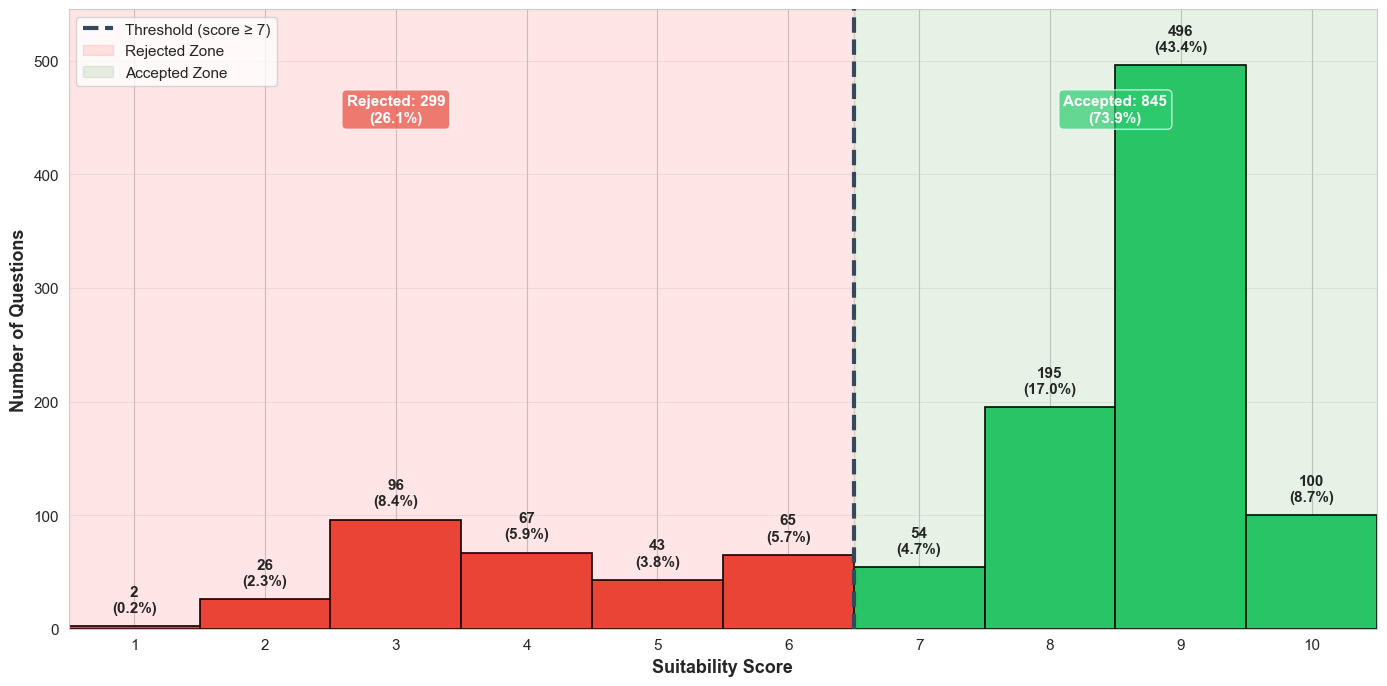
\includegraphics[width=1.0\linewidth]{figs/ch4/4.1/distribution-of-suitability.png}
    \caption{Distribution of Suitability Scores}
    \label{fig:distribution-of-suitability}
\end{figure}

Figure \ref{fig:osq-conversion-category-distribution} summarizes the number of questions accepted for conversion and rejected across each Systems Engineering category and sub-category represented in the SysEngBench dataset. Categories are listed on the vertical axis, ordered by total question count, while the horizontal axis denotes the number of questions. For each category, green bars indicate questions that met the suitability threshold and were successfully converted, while red bars indicate questions rejected during the filtering process.

Substantial variation in the number of questions per category can be observed. Several categories contain relatively large question pools, such as Design Standards, DODAF, Requirements, and Project Management. Within these categories, both accepted and rejected questions appear, with total counts ranging from approximately 50 to over 90. Mid-sized categories such as Use Cases, Activity Diagrams, Sequence Diagrams, Parametric Diagrams, and Requirements Diagrams contain between 10 and 30 questions each, again with both accepted and rejected items.

A wide range of smaller categories is also present, many containing fewer than 10 questions. These include technical areas such as Fault Tree Analysis, Maintainability Demonstration, Usability, Environmental Considerations, among other topics. Across these categories, the distribution of accepted and rejected questions varies, with some categories showing only a small number of accepted items and others showing a near-balanced split.

\begin{figure}[htbp]
    \centering
    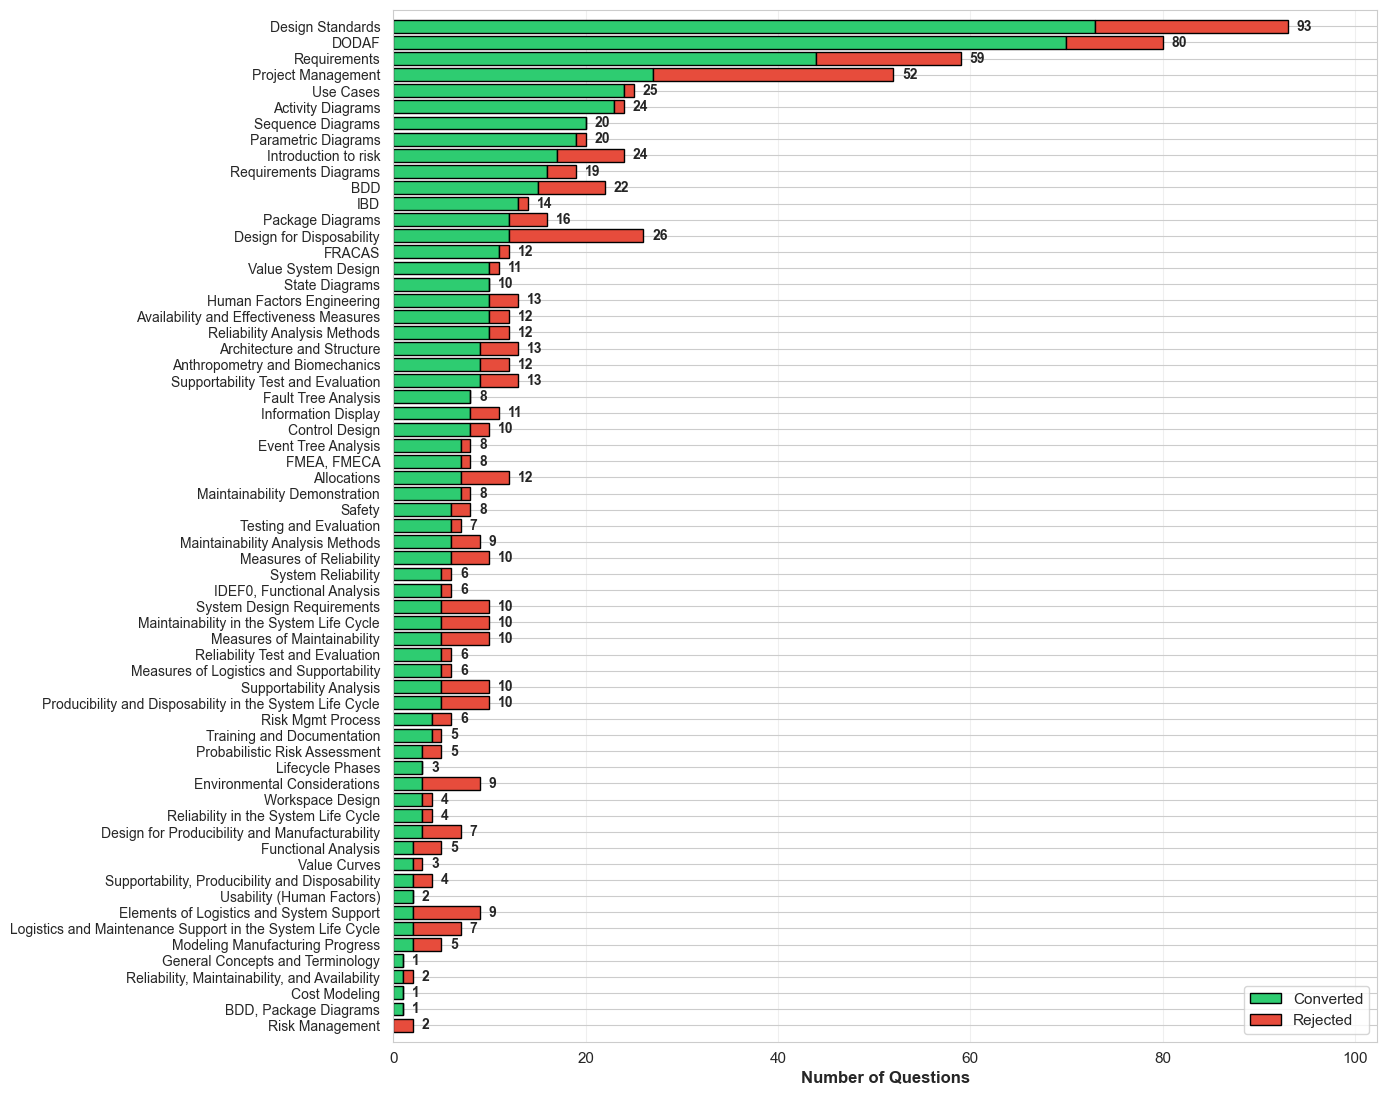
\includegraphics[width=1\linewidth]{figs/ch4/4.1/osq-conversion-category-distribution.png}
    \caption{Sub-Category Level Distribution of Converted and Rejected SysEngBench Questions}
    \label{fig:osq-conversion-category-distribution}
\end{figure}

% \newpage
\clearpage
\section{Performance on Multiple Choice Questions}\label{sec:performance_mcq}

Figure \ref{fig:mcq_position_heatmap} displays a heatmap of \ac{mcq} accuracy for each model across the four answer-key positions (A, B, C, and D). Models are listed on the vertical axis sorted in descending order of average per-position accuracy, while the horizontal axis corresponds to the correct answer position. The color scale reflects accuracy values between 0.70 and 1.00, with darker greens indicating higher accuracy and shades moving toward yellow or red representing lower accuracy.

The \acp{mcq} included consist only of the subset of questions that passed the suitability filtering process and therefore have a corresponding \ac{osq} equivalent. This subset of converted \acp{mcq} represents the portion of the dataset that is used for both \ac{mcq} and \ac{osq} evaluation, and reflects only those questions eligible for direct cross-modality comparison.

Across the models, accuracy values range from approximately 0.56 to 0.97. Several models show consistently high accuracy across all four positions, with the highest values occurring in the upper rows of the heatmap. Mid-tier models exhibit moderate accuracy with small variations between positions. Lower-accuracy models display more pronounced variation between positions and include several cells shaded in orange or red. Individual accuracy values are printed within each cell for reference.

\begin{figure}
    \centering
    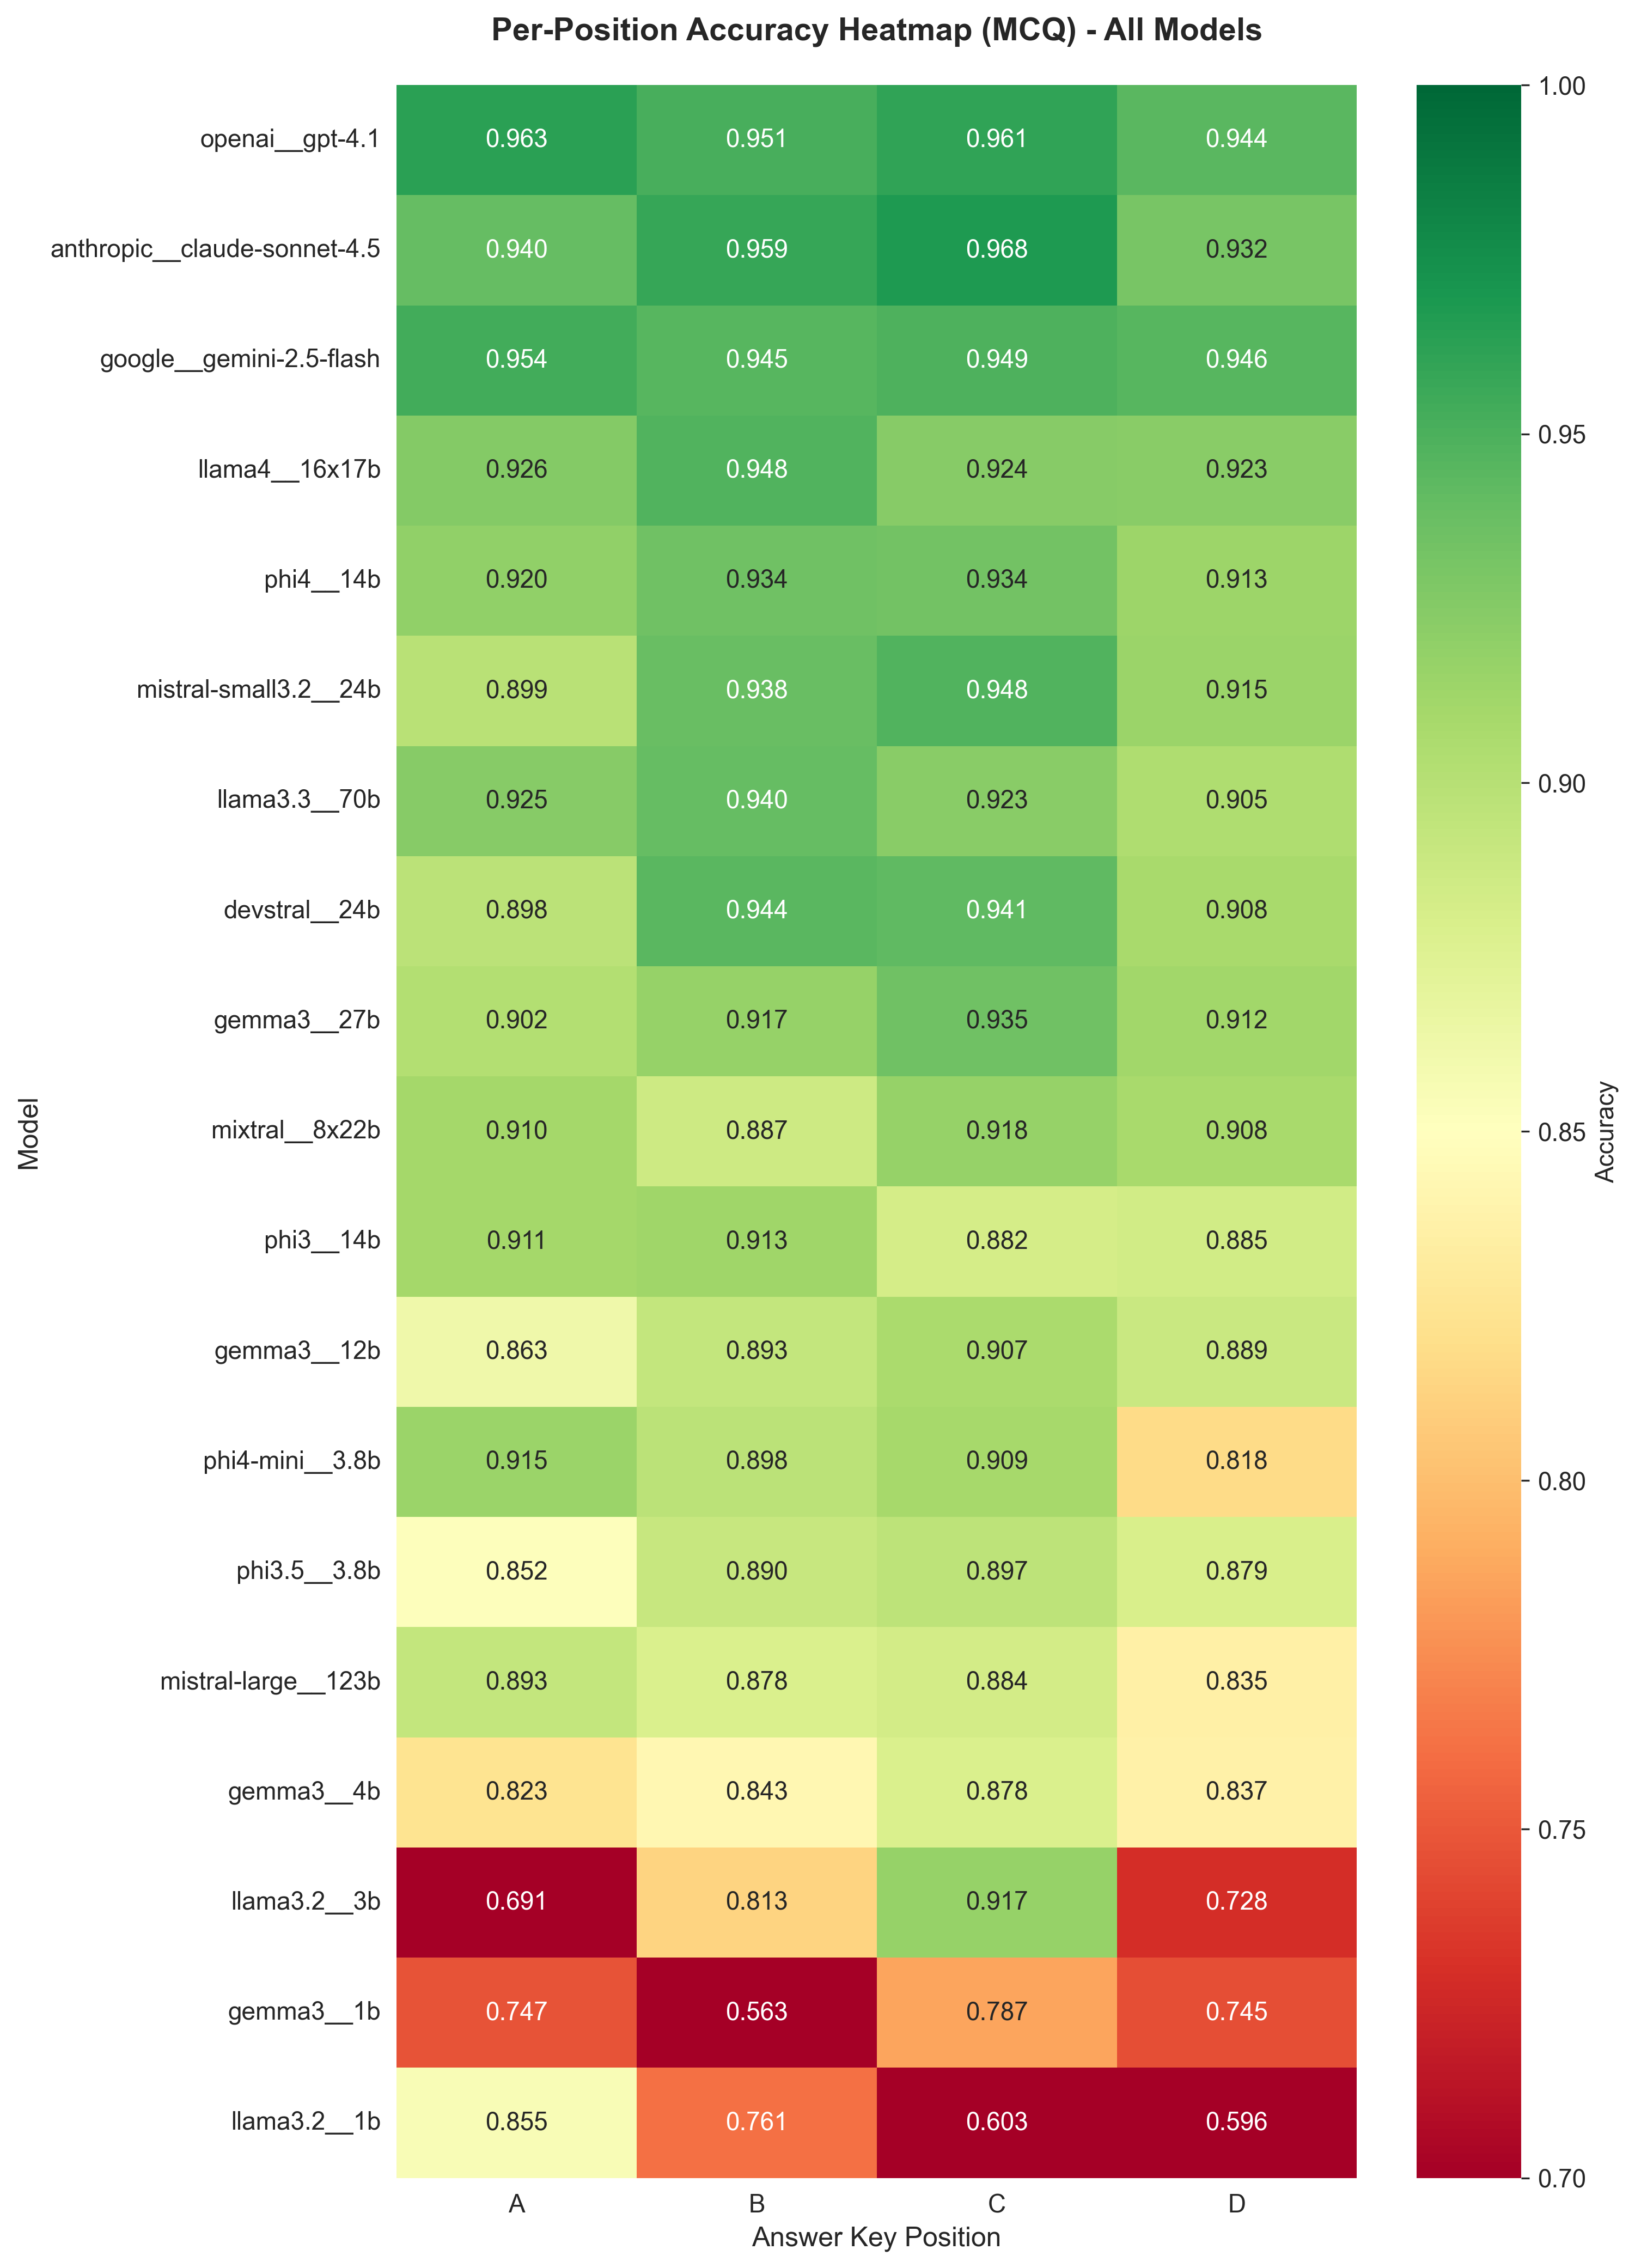
\includegraphics[width=0.75\linewidth]{figs/ch4/4.2/mcq_position_heatmap.png}
    \caption{MCQ Per-Position Heatmap}
    \label{fig:mcq_position_heatmap}
\end{figure}

Bootstrap confidence intervals work by repeatedly remixing the existing test data (sampling with replacement) to see how much the result—like accuracy—would change if one had gotten a slightly different test set. The spread of those results gives an estimate of how uncertain your measured accuracy is, shown as the little error bars in the chart.

Figure \ref{fig:mcq_bootstrap_ci} presents \ac{mcq} accuracy for all evaluated models along with 95\% bootstrap confidence intervals. Models are ordered from lowest to highest accuracy along the horizontal axis, and the vertical axis shows accuracy on a scale from 0.50 to 1.00. Each point represents the mean accuracy estimate for a model, and the accompanying vertical error bars indicate the lower and upper bounds of the corresponding bootstrap interval.

The bootstrap method used involves repeatedly resampling the evaluation set with replacement to generate many synthetic samples of equal size. Accuracy is computed on each resampled dataset, and the resulting distribution of values is used to derive the confidence interval. This provides an empirical estimate of uncertainty around each model's accuracy without imposing assumptions about the underlying distribution of responses.

Accuracy values span a range from approximately 0.69 to 0.95 across models. Lower-accuracy models show wider-spread error bars in the lower portion of the figure, while higher-accuracy models appear clustered near the upper portion with intervals that remain relatively narrow. The spacing between points indicates an increase in accuracy from left to right. The plot provides a summary of accuracy estimates together with the associated uncertainty for each model under the \ac{mcq} variation evaluation procedure.

\begin{figure}[htbp]
    \centering
    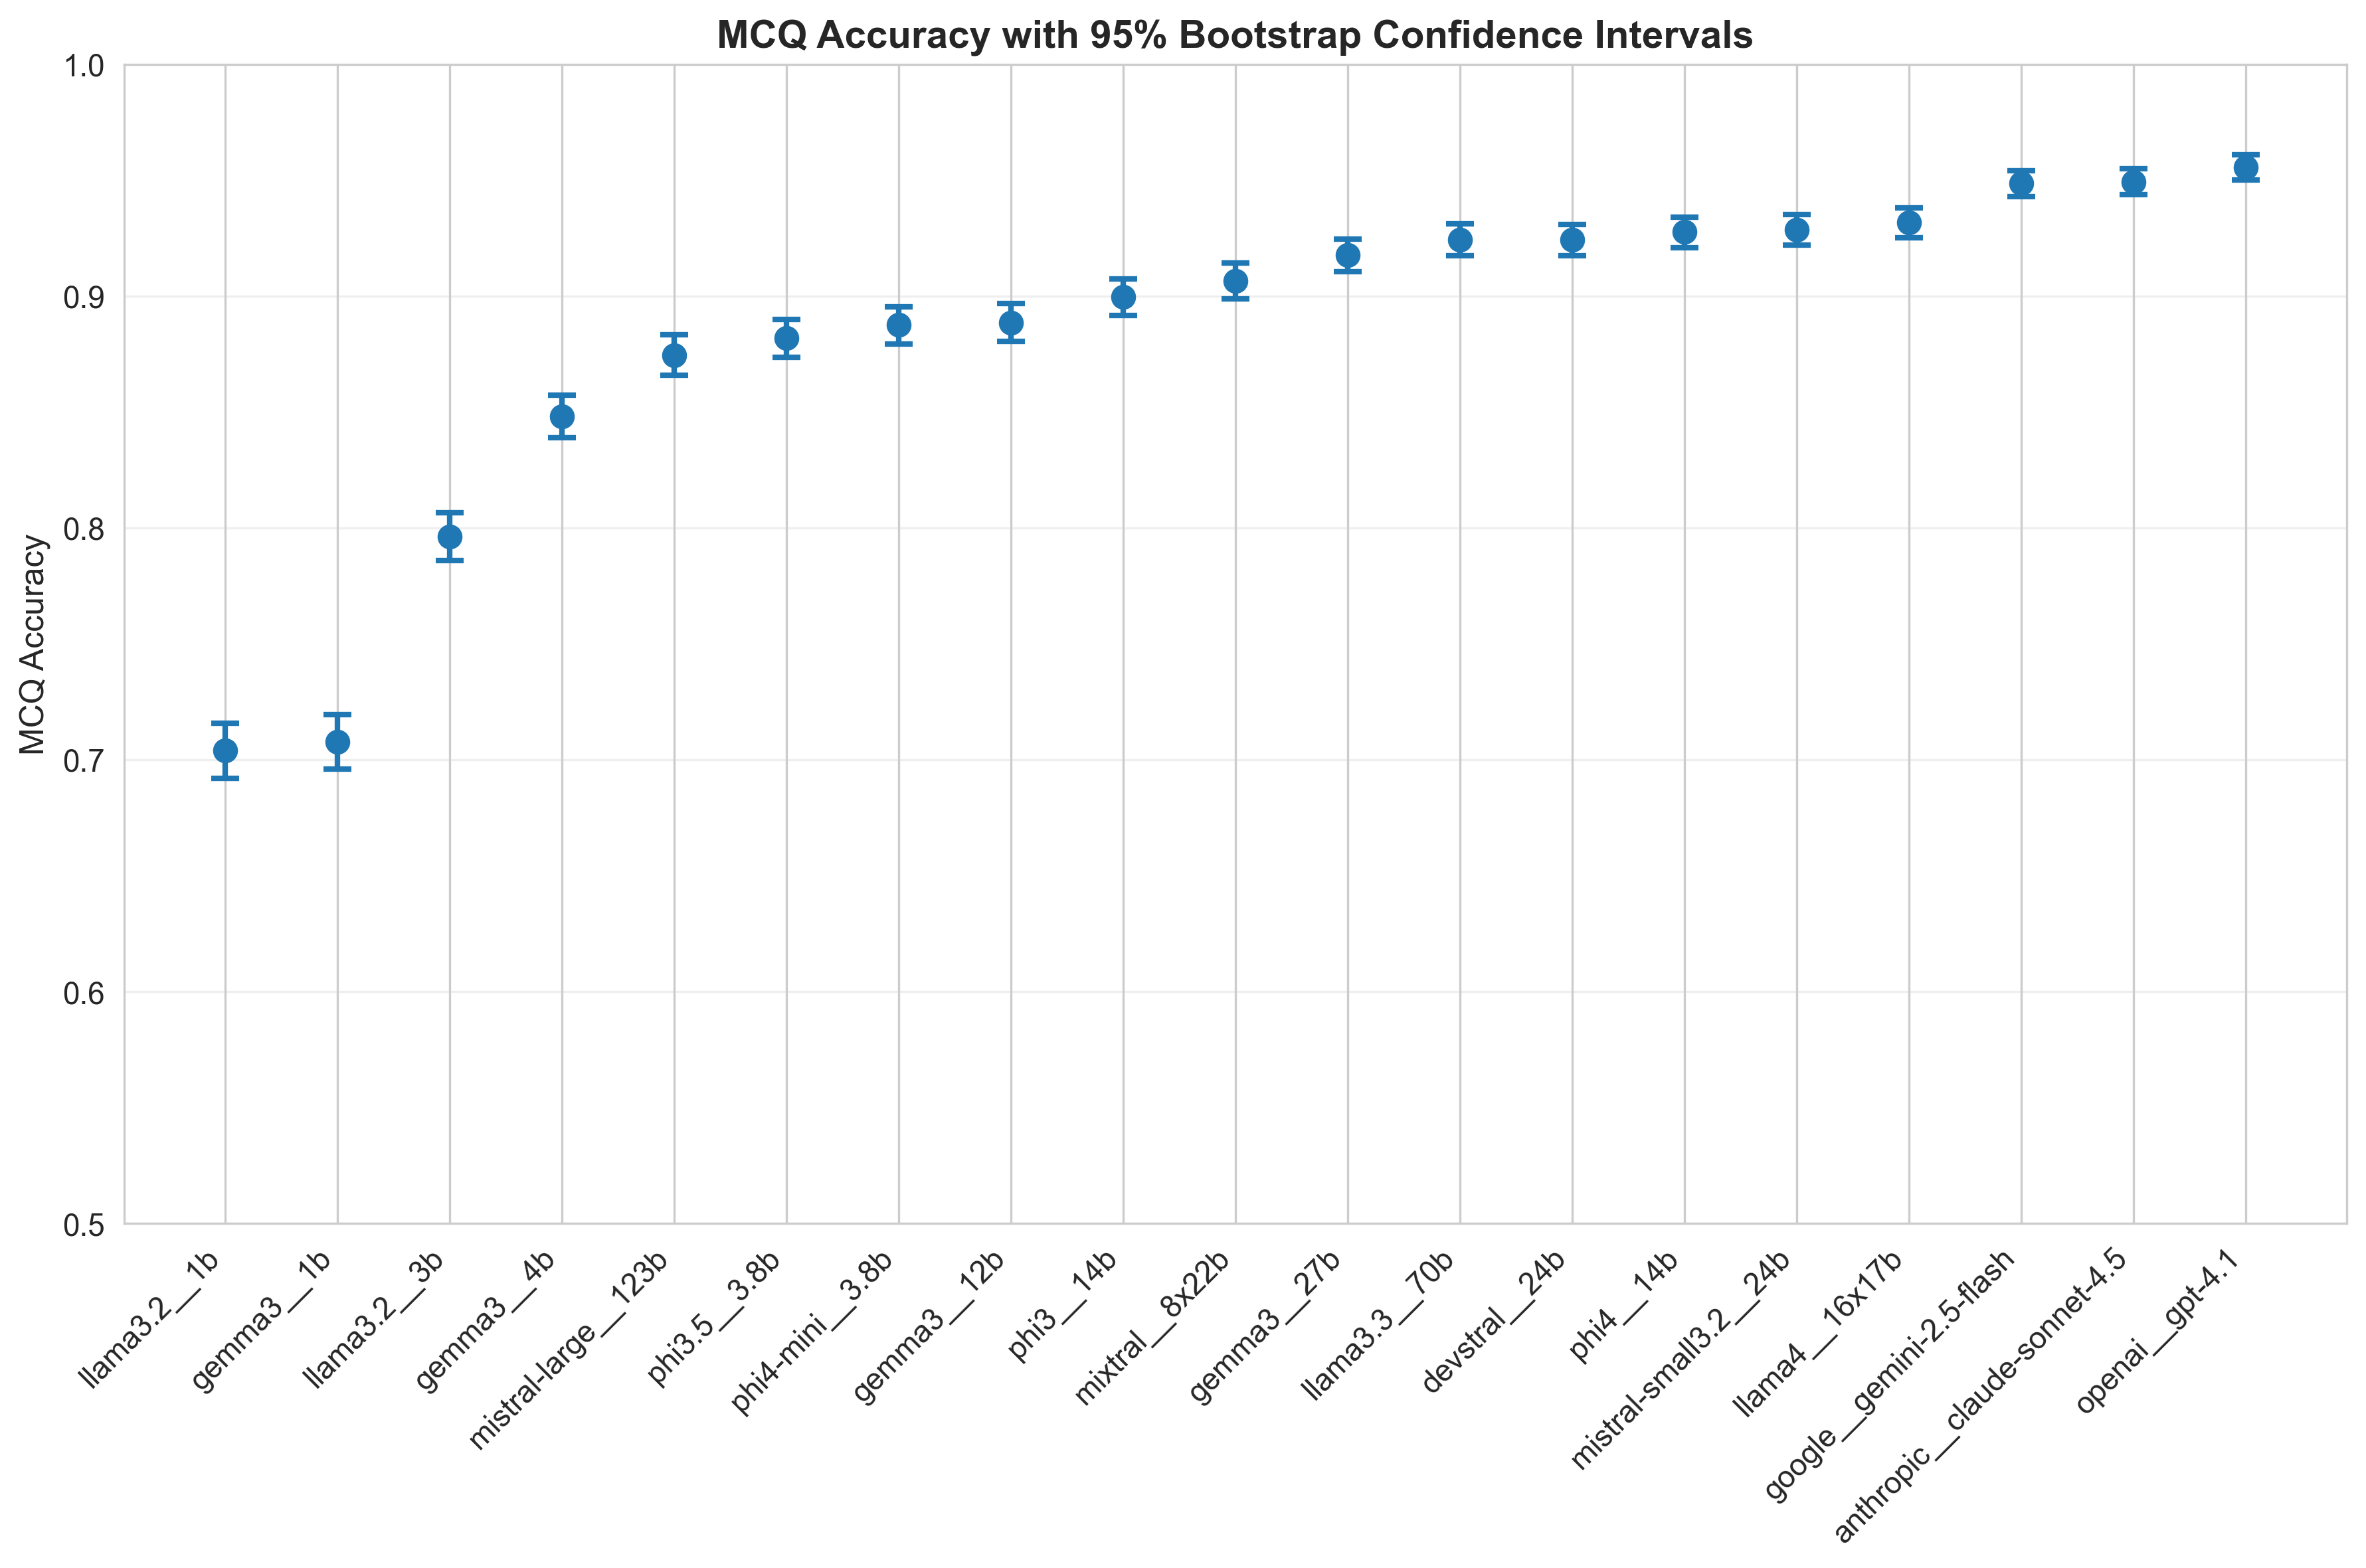
\includegraphics[width=1\linewidth]{figs/ch4/4.2/mcq_bootstrap_ci.png}
    \caption{MCQ Bootstrap Confidence Intervals}
    \label{fig:mcq_bootstrap_ci}
\end{figure}

\subsection{Position Bias Statistical Analysis}

To quantify position bias, chi-square tests of independence were conducted for each model, testing whether the distribution of correct responses was independent of answer position. Table \ref{tab:chi_square_position} presents the chi-square statistic, $p$-value, Cramér's V effect size, and significance determination for each model.

\begin{table}[htbp]
\centering
\caption{Chi-Square Test Results for Position Bias}
\label{tab:chi_square_position}
\begin{tabular}{lrrrr}
\toprule
Model & $\chi^2$ stat & $p$-value & Cramér's $V$ & Significant \\
\midrule
\texttt{anthropic\_\_claude-sonnet-4.5} & 19.69 & 0.0006 & 0.059 & Yes \\
\texttt{devstral\_\_24b} & 27.50 & $<$0.0001 & 0.069 & Yes \\
\texttt{gemma3\_\_12b} & 12.09 & 0.0167 & 0.046 & Yes \\
\texttt{gemma3\_\_1b} & 167.35 & $<$0.0001 & 0.171 & Yes \\
\texttt{gemma3\_\_27b} & 9.24 & 0.0554 & 0.040 & No \\
\texttt{gemma3\_\_4b} & 16.17 & 0.0028 & 0.053 & Yes \\
\texttt{google\_\_gemini-2.5-flash} & 1.13 & 0.8901 & 0.014 & No \\
\texttt{llama3.2\_\_1b} & 262.77 & $<$0.0001 & 0.214 & Yes \\
\texttt{llama3.2\_\_3b} & 224.04 & $<$0.0001 & 0.198 & Yes \\
\texttt{llama3.3\_\_70b} & 10.56 & 0.0320 & 0.043 & Yes \\
\texttt{llama4\_\_16x17b} & 8.81 & 0.0661 & 0.039 & No \\
\texttt{mistral-large\_\_123b} & 21.78 & 0.0002 & 0.062 & Yes \\
\texttt{mistral-small3.2\_\_24b} & 30.47 & $<$0.0001 & 0.073 & Yes \\
\texttt{mixtral\_\_8x22b} & 7.11 & 0.1300 & 0.035 & No \\
\texttt{openai\_\_gpt-4.1} & 6.73 & 0.1507 & 0.034 & No \\
\texttt{phi3.5\_\_3.8b} & 13.91 & 0.0076 & 0.049 & Yes \\
\texttt{phi3\_\_14b} & 11.45 & 0.0219 & 0.045 & Yes \\
\texttt{phi4-mini\_\_3.8b} & 71.64 & $<$0.0001 & 0.112 & Yes \\
\texttt{phi4\_\_14b} & 7.43 & 0.1148 & 0.036 & No \\
\bottomrule
\end{tabular}
\end{table}

Additionally, Friedman tests were conducted as a non-parametric repeated-measures analysis, treating each question as a subject measured across four conditions (answer positions A, B, C, D). Table \ref{tab:friedman_position} presents the Friedman test statistic, $p$-value, Kendall's W effect size, and significance for each model. Kendall's W ranges from 0 to 1, where values near 0 indicate no agreement (i.e., random variation across positions) and values near 1 indicate perfect agreement.

\begin{table}[htbp]
\centering
\caption{Friedman Test Results for Position Bias}
\label{tab:friedman_position}
\begin{tabular}{lrrrr}
\toprule
Model & Friedman $\chi^2$ & $p$-value & Kendall's $W$ & Significant \\
\midrule
\texttt{anthropic\_\_claude-sonnet-4.5} & 46.24 & $<$0.0001 & 0.014 & Yes \\
\texttt{devstral\_\_24b} & 58.15 & $<$0.0001 & 0.017 & Yes \\
\texttt{gemma3\_\_12b} & 30.72 & $<$0.0001 & 0.009 & Yes \\
\texttt{gemma3\_\_1b} & 285.10 & $<$0.0001 & 0.083 & Yes \\
\texttt{gemma3\_\_27b} & 22.72 & $<$0.0001 & 0.007 & Yes \\
\texttt{gemma3\_\_4b} & 38.89 & $<$0.0001 & 0.011 & Yes \\
\texttt{google\_\_gemini-2.5-flash} & 3.48 & 0.3238 & 0.001 & No \\
\texttt{llama3.2\_\_1b} & 446.62 & $<$0.0001 & 0.130 & Yes \\
\texttt{llama3.2\_\_3b} & 387.90 & $<$0.0001 & 0.113 & Yes \\
\texttt{llama3.3\_\_70b} & 27.95 & $<$0.0001 & 0.008 & Yes \\
\texttt{llama4\_\_16x17b} & 21.64 & 0.0001 & 0.006 & Yes \\
\texttt{mistral-large\_\_123b} & 43.74 & $<$0.0001 & 0.013 & Yes \\
\texttt{mistral-small3.2\_\_24b} & 58.84 & $<$0.0001 & 0.017 & Yes \\
\texttt{mixtral\_\_8x22b} & 17.24 & 0.0006 & 0.005 & Yes \\
\texttt{openai\_\_gpt-4.1} & 20.47 & 0.0001 & 0.006 & Yes \\
\texttt{phi3.5\_\_3.8b} & 37.23 & $<$0.0001 & 0.011 & Yes \\
\texttt{phi3\_\_14b} & 23.15 & $<$0.0001 & 0.007 & Yes \\
\texttt{phi4-mini\_\_3.8b} & 149.70 & $<$0.0001 & 0.044 & Yes \\
\texttt{phi4\_\_14b} & 15.00 & 0.0018 & 0.004 & Yes \\
\bottomrule
\end{tabular}
\end{table}

\begin{figure}[htbp]
    \centering
    
\includegraphics[width=1\linewidth]{figs/ch4/fig_cramers_v_position_bias.png}
    \caption{Cramér's V Position Bias Effect Sizes}
    \label{fig:mcq_cramers_v}
\end{figure}

Figure \ref{fig:mcq_cramers_v} presents position bias effect, quantified using Cramér's V, which measures the strength of association between answer choice position and the model's selected response in \acp{mcq}. Each horizontal bar corresponds to a model, with the x-axis indicating the magnitude of the effect size and the y-axis listing models sorted from highest to lowest bias, top to bottom. Larger values of Cramér's V indicate stronger dependence on option position, while values near zero indicate little to no position bias.

Color coding and reference lines provide interpretive structure for these effect sizes. Green bars denote models whose position bias falls in the negligible range, while orange bars indicate models exceeding the conventional threshold for a small effect (approximately Cramér's V = 0.10). Vertical dashed lines mark standard benchmarks for small and medium-to-large effects. Notably, while several models exceed the small-effect threshold, none approach the medium or large effect range.

Interpreting these results collectively: while 13 of 19 models show statistically significant position bias according to the chi-square test, the effect sizes (Cramér's V) remain small to negligible in most cases. Only the smallest models (\texttt{llama3.2\_\_1b}, \texttt{llama3.2\_\_3b}, \texttt{gemma3\_\_1b}, and \texttt{phi4-mini\_\_3.8b}) exceed the 0.10 threshold for a small effect, suggesting that position bias is primarily a concern for smaller-capacity models. Larger models such as \texttt{google\_\_gemini-2.5-flash}, \texttt{openai\_\_gpt-4.1}, and \texttt{gemma3\_\_27b} show no statistically significant position bias.

% \newpage
\clearpage
\section{Performance on Open Style Questions}\label{sec:performance_osq}

Figure \ref{fig:osq_violin_scores} presents violin plots of OSQ total scores for each model, showing the distributional shape, central tendency, and spread of scores. Models appear along the horizontal axis, and OSQ total scores are plotted on the vertical axis. Within each violin, a filled density shape depicts the distribution of scores, while an embedded box plot indicates the inter-quartile range, median, and approximate extrema. A horizontal dashed red line marks the passing threshold of 70 points.

Across models, the widths of the violins vary, indicating differences in score dispersion. Some models display narrow, high-centered distributions, while others present wider shapes with scores spanning a larger range. Several violins extend below the passing threshold, while others remain predominantly above.

The violins are constructed using kernel density estimation (KDE), which Seaborn computes independently for each language model using a Gaussian kernel and standard bandwidth selection. As Gaussian kernels have unbounded support, the density estimate can extend slightly below 0 or above 100 while all underlying rubric-assigned OSQ scores lie strictly within the 0–100 scoring range. The vertical extent of each violin therefore reflects both the observed score distribution and the smooth KDE-based interpolation used to visualize it.

The figure provides a model-by-model comparison of OSQ score distributions, illustrating the central scoring tendencies and the degree of variability in OSQ performance across all evaluated models.

\begin{figure}[htbp]
    \centering
    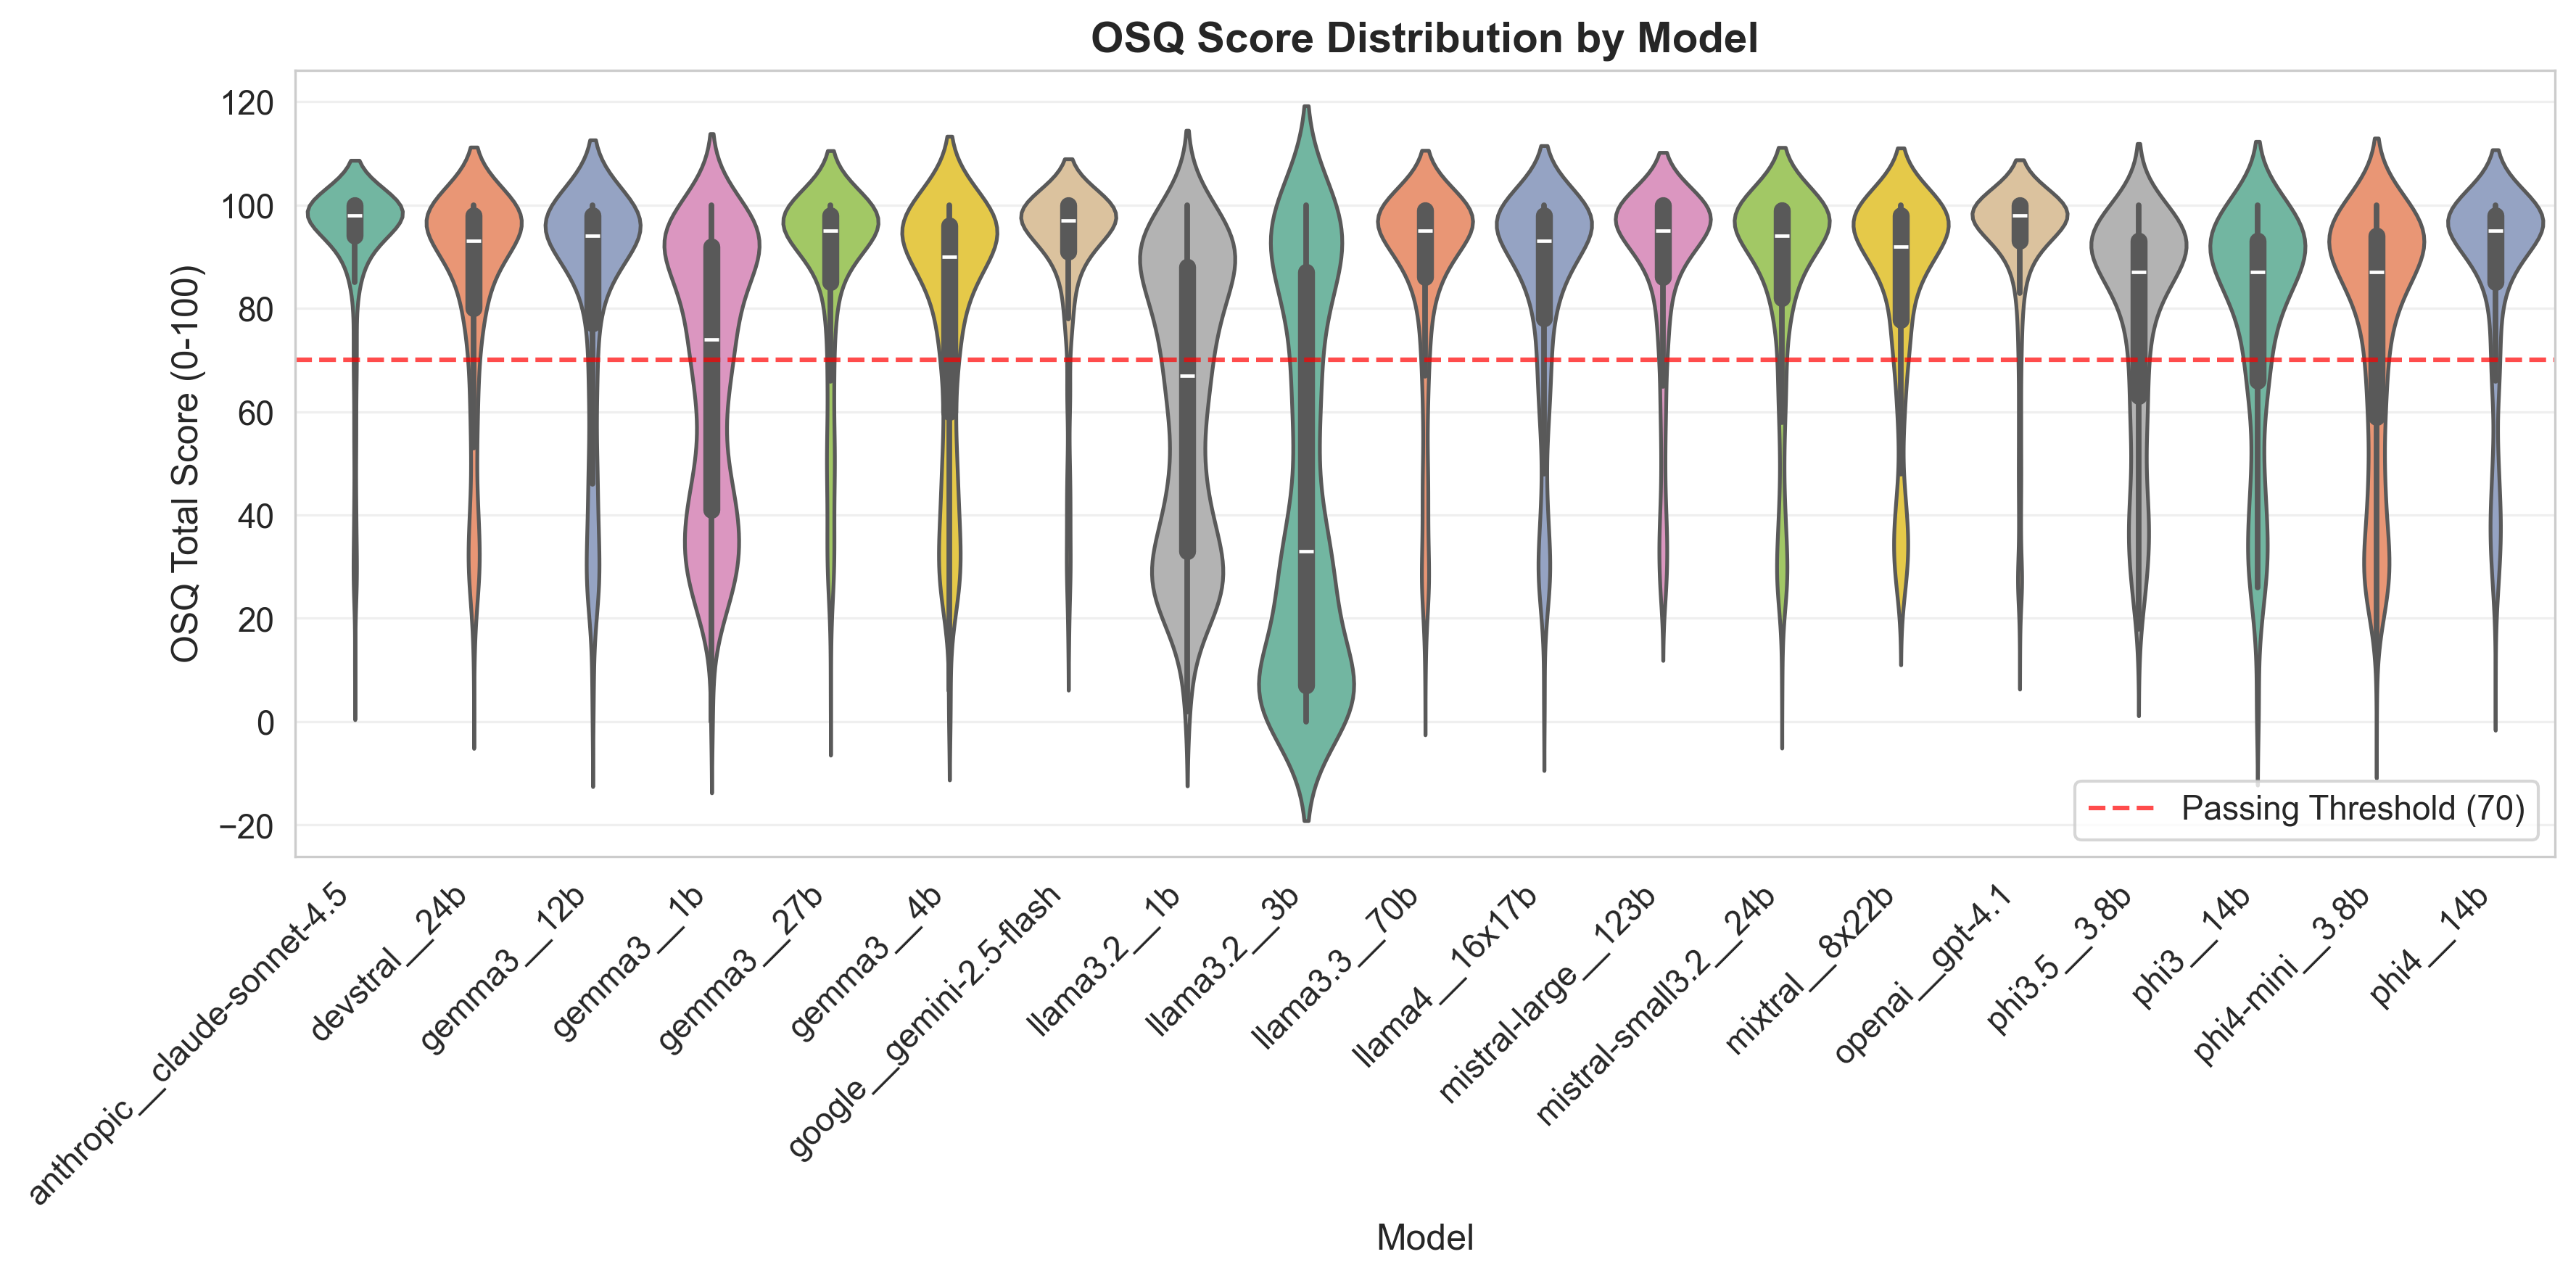
\includegraphics[width=1\linewidth]{figs/ch4/4.3/osq_violin_scores.png}
    \caption{OSQ Score Distributions by Model (Violin Plot)}
    \label{fig:osq_violin_scores}
\end{figure}

Figure \ref{fig:osq_score_histogram} displays kernel density estimates (KDEs) of total \ac{osq} scores for all evaluated models. Each curve represents the estimated score distribution for a single model, with OSQ total scores plotted along the horizontal axis and density values shown on the vertical axis. A vertical dashed red line indicates the passing threshold of 70 points.

The KDE curves were generated using the default Gaussian kernel in Seaborn with standard bandwidth selection, applied independently to each model's distribution of OSQ scores. Gaussian kernels extend smoothly beyond the minimum and maximum observed values, the resulting density curves may extend slightly below 0 or above 100 even though all underlying rubric scores fall within the 0–100 range. The vertical axis represents probability density rather than counts, and therefore the area under each curve integrates to 1 for each model.

Across models, the density curves exhibit varied shapes, spreads, and peak locations, reflecting differences in score distributions. Some models show narrow, high-centered curves, whereas others display wider or multi-modal distributions. The figure provides an aggregate visualization of OSQ total score distributions and their relation to the passing threshold across all evaluated models.

\begin{figure}[htbp]
    \centering
    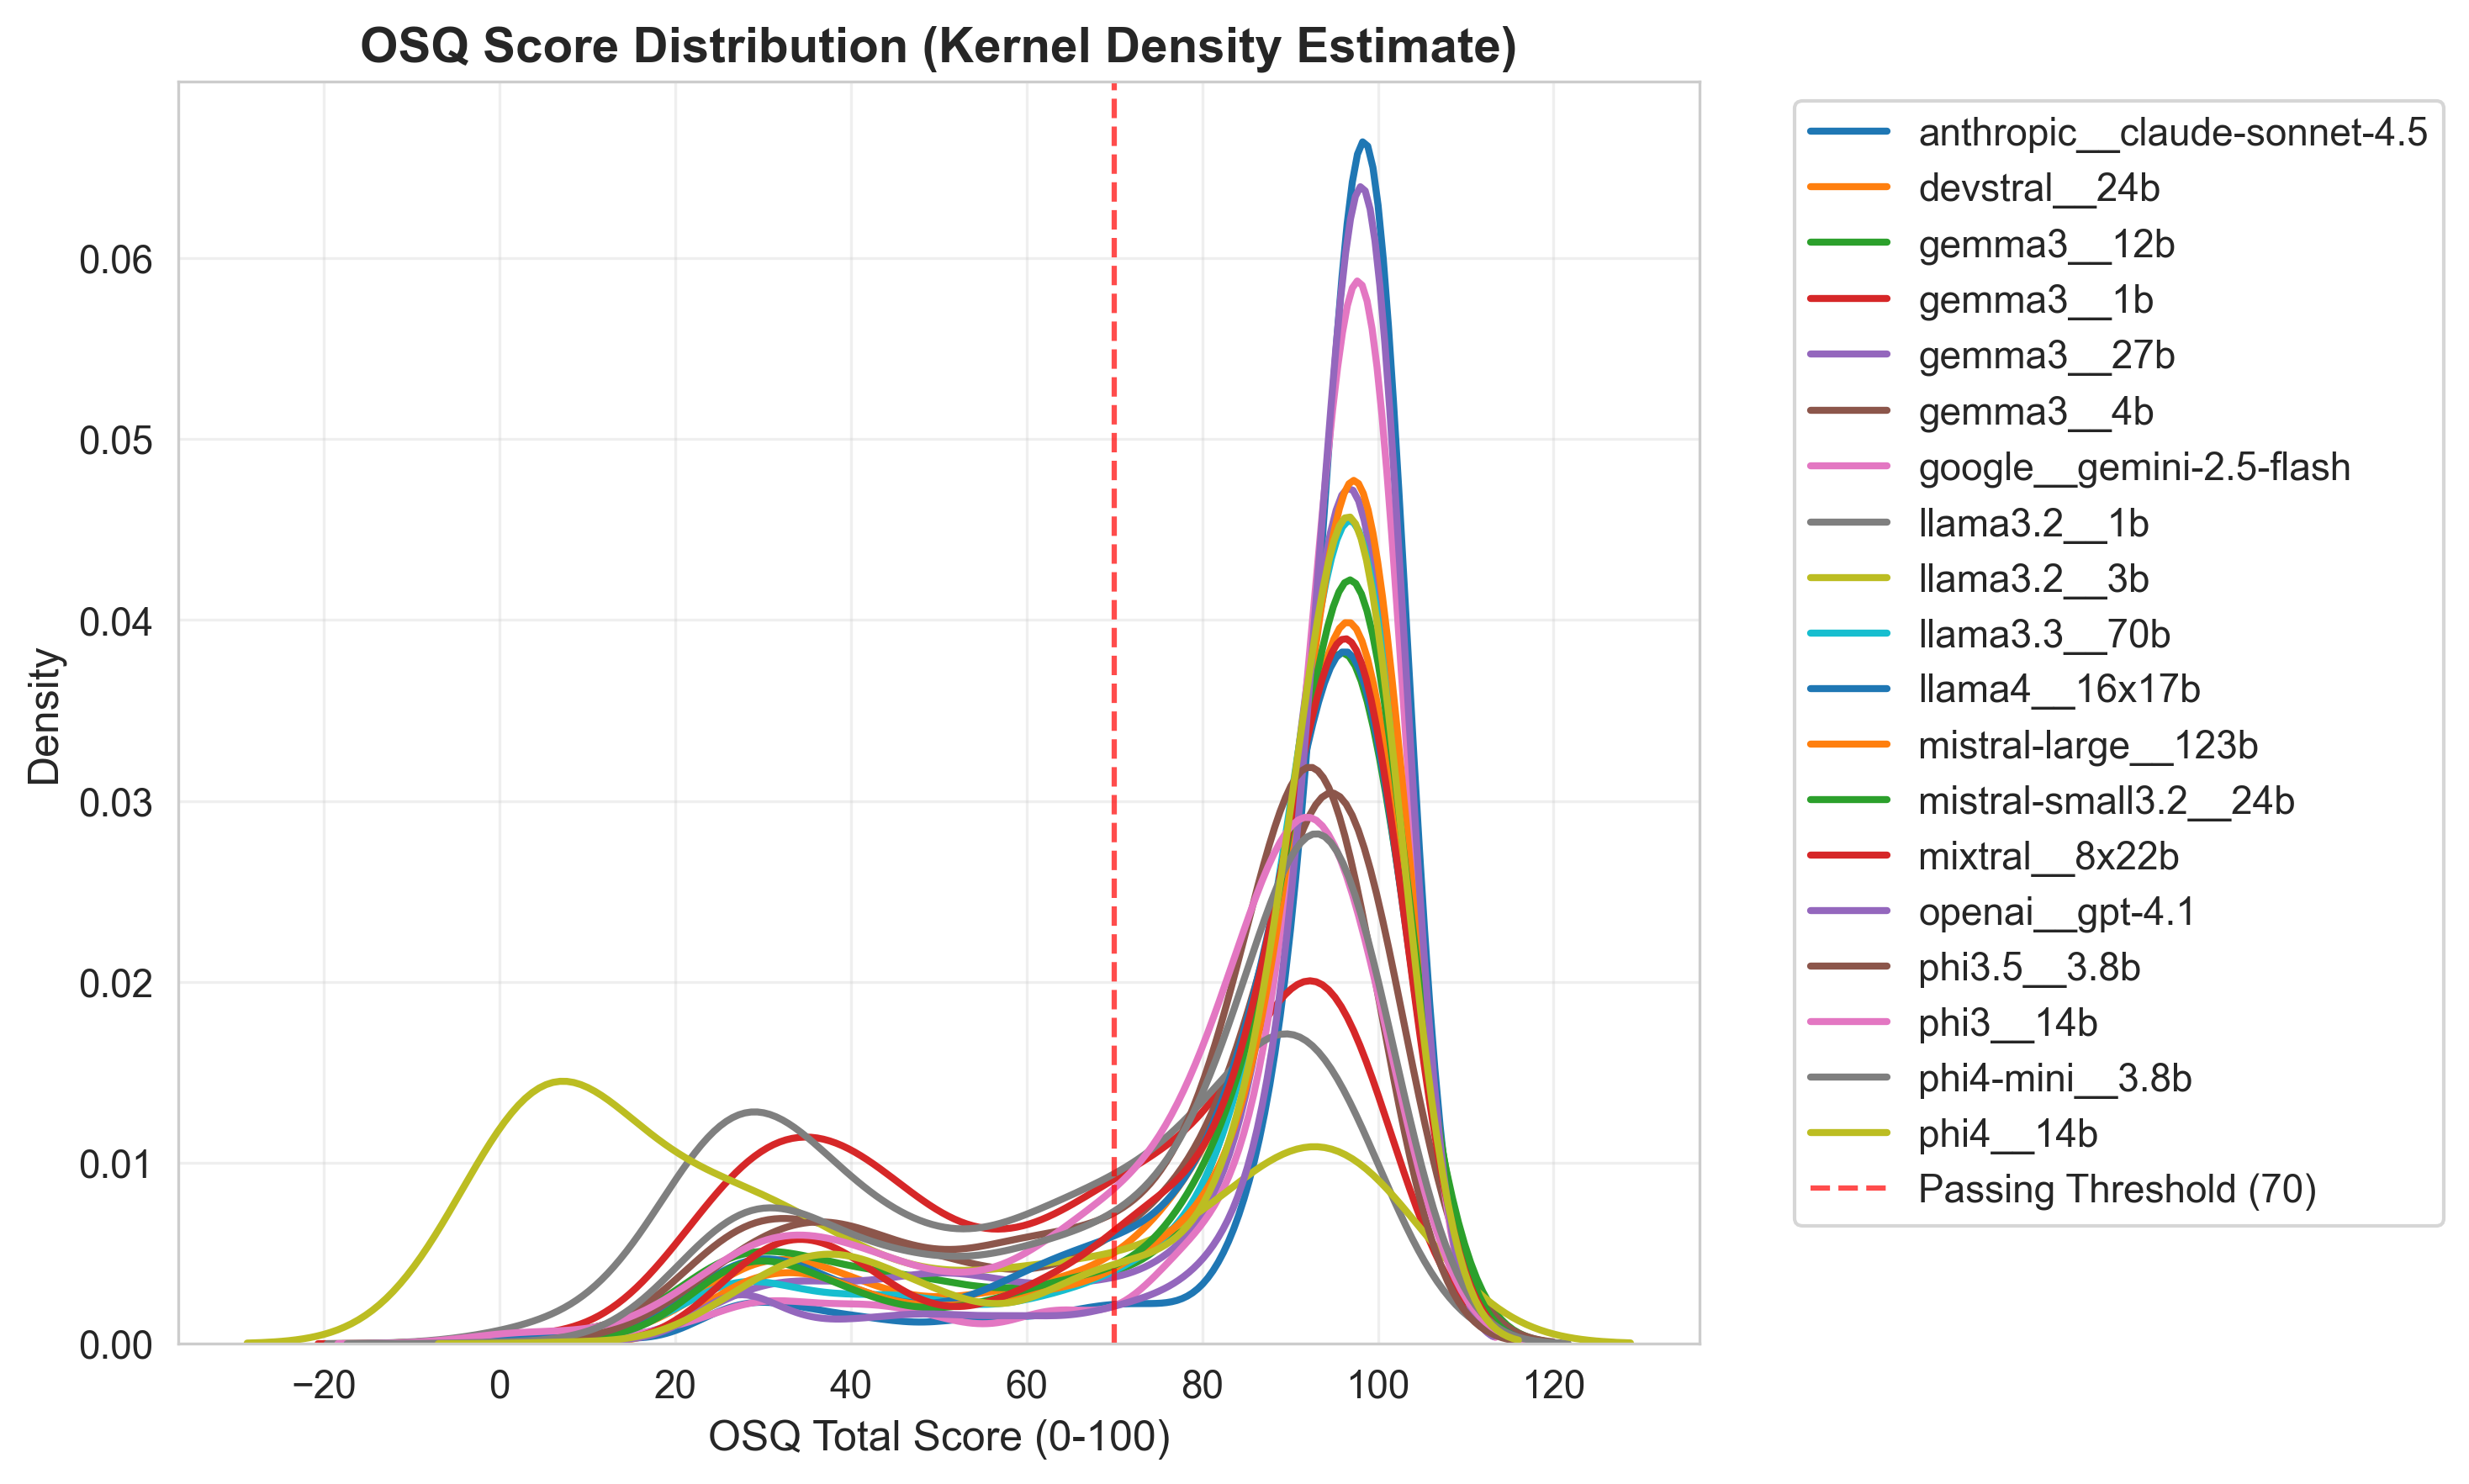
\includegraphics[width=1\linewidth]{figs/ch4/4.3/osq_score_histogram.png}
    \caption{OSQ Score Distribution, Kernel Density Estimate}
    \label{fig:osq_score_histogram}
\end{figure}

\subsection{Inter-Judge Agreement}

To validate the reliability of the LLM-as-a-judge methodology, inter-judge agreement was assessed using Spearman's rank correlation between two independent judge models: GPT-OSS (120B parameters) and OpenAI GPT-5-mini. The correlation was computed across all 16,051 judged samples where both judges provided scores.

The analysis revealed a Spearman's $\rho$ of 0.901 ($p < 0.0001$), indicating very strong agreement between the two judge models. This high correlation suggests that the rubric-based scoring approach yields consistent evaluations regardless of which LLM serves as the judge, supporting the validity of the OSQ scoring methodology.

\subsection{Rubric Dimension Analysis}

OSQ responses were evaluated across five rubric dimensions, each scored on a 0–20 scale: \emph{Technical Accuracy}, \emph{Conceptual Understanding}, \emph{Completeness}, \emph{Clarity and Organization}, and \emph{Professional Relevance}. Figure \ref{fig:osq_rubric_dimensions} presents the mean scores across these dimensions for all evaluated models.

\begin{figure}[htbp]
    \centering
    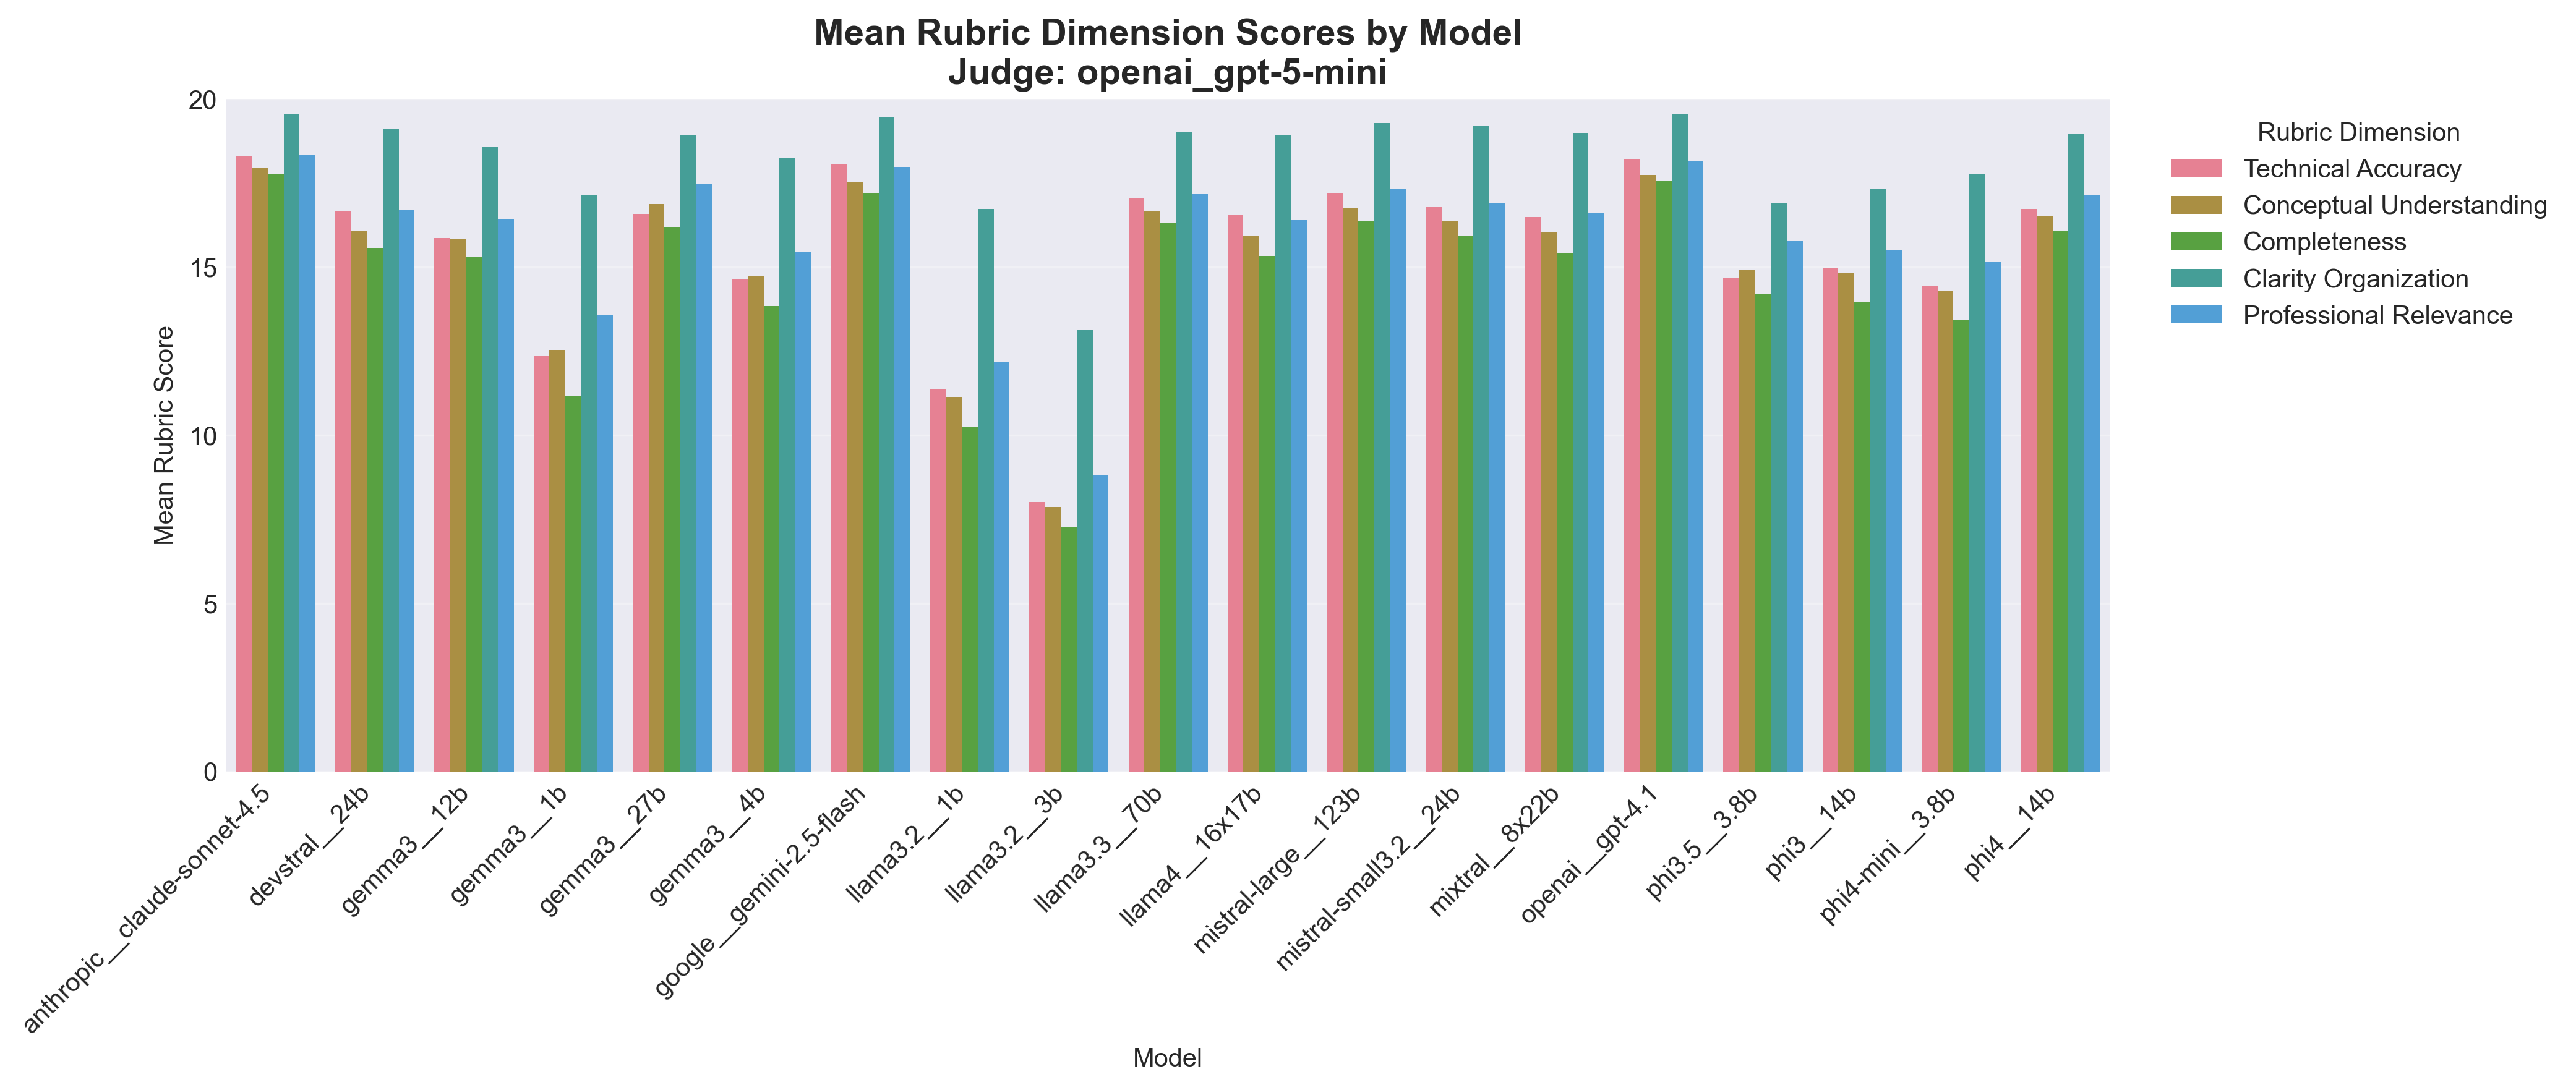
\includegraphics[width=1\linewidth]{figs/ch4/4.3/osq_rubric_dimensions_openai_gpt-5-mini.png}
    \caption{OSQ Rubric Dimension Scores by Model}
    \label{fig:osq_rubric_dimensions}
\end{figure}

The rubric dimension breakdown reveals that models generally perform most strongly on \emph{Professional Relevance} and \emph{Clarity and Organization}, while showing more variation on \emph{Technical Accuracy} and \emph{Completeness}. This pattern suggests that while LLMs can effectively communicate in a professional manner, they may struggle more with domain-specific technical precision and comprehensive coverage of all required elements.

\subsection{Bootstrap Confidence Intervals for OSQ Scores}

Figure \ref{fig:osq_bootstrap_ci} presents 95\% bootstrap confidence intervals for mean OSQ scores across all evaluated models. Bootstrap resampling (n=1,000 iterations) was used to estimate the uncertainty around each model's mean score without assuming normality of the underlying score distribution.

\begin{figure}[htbp]
    \centering
    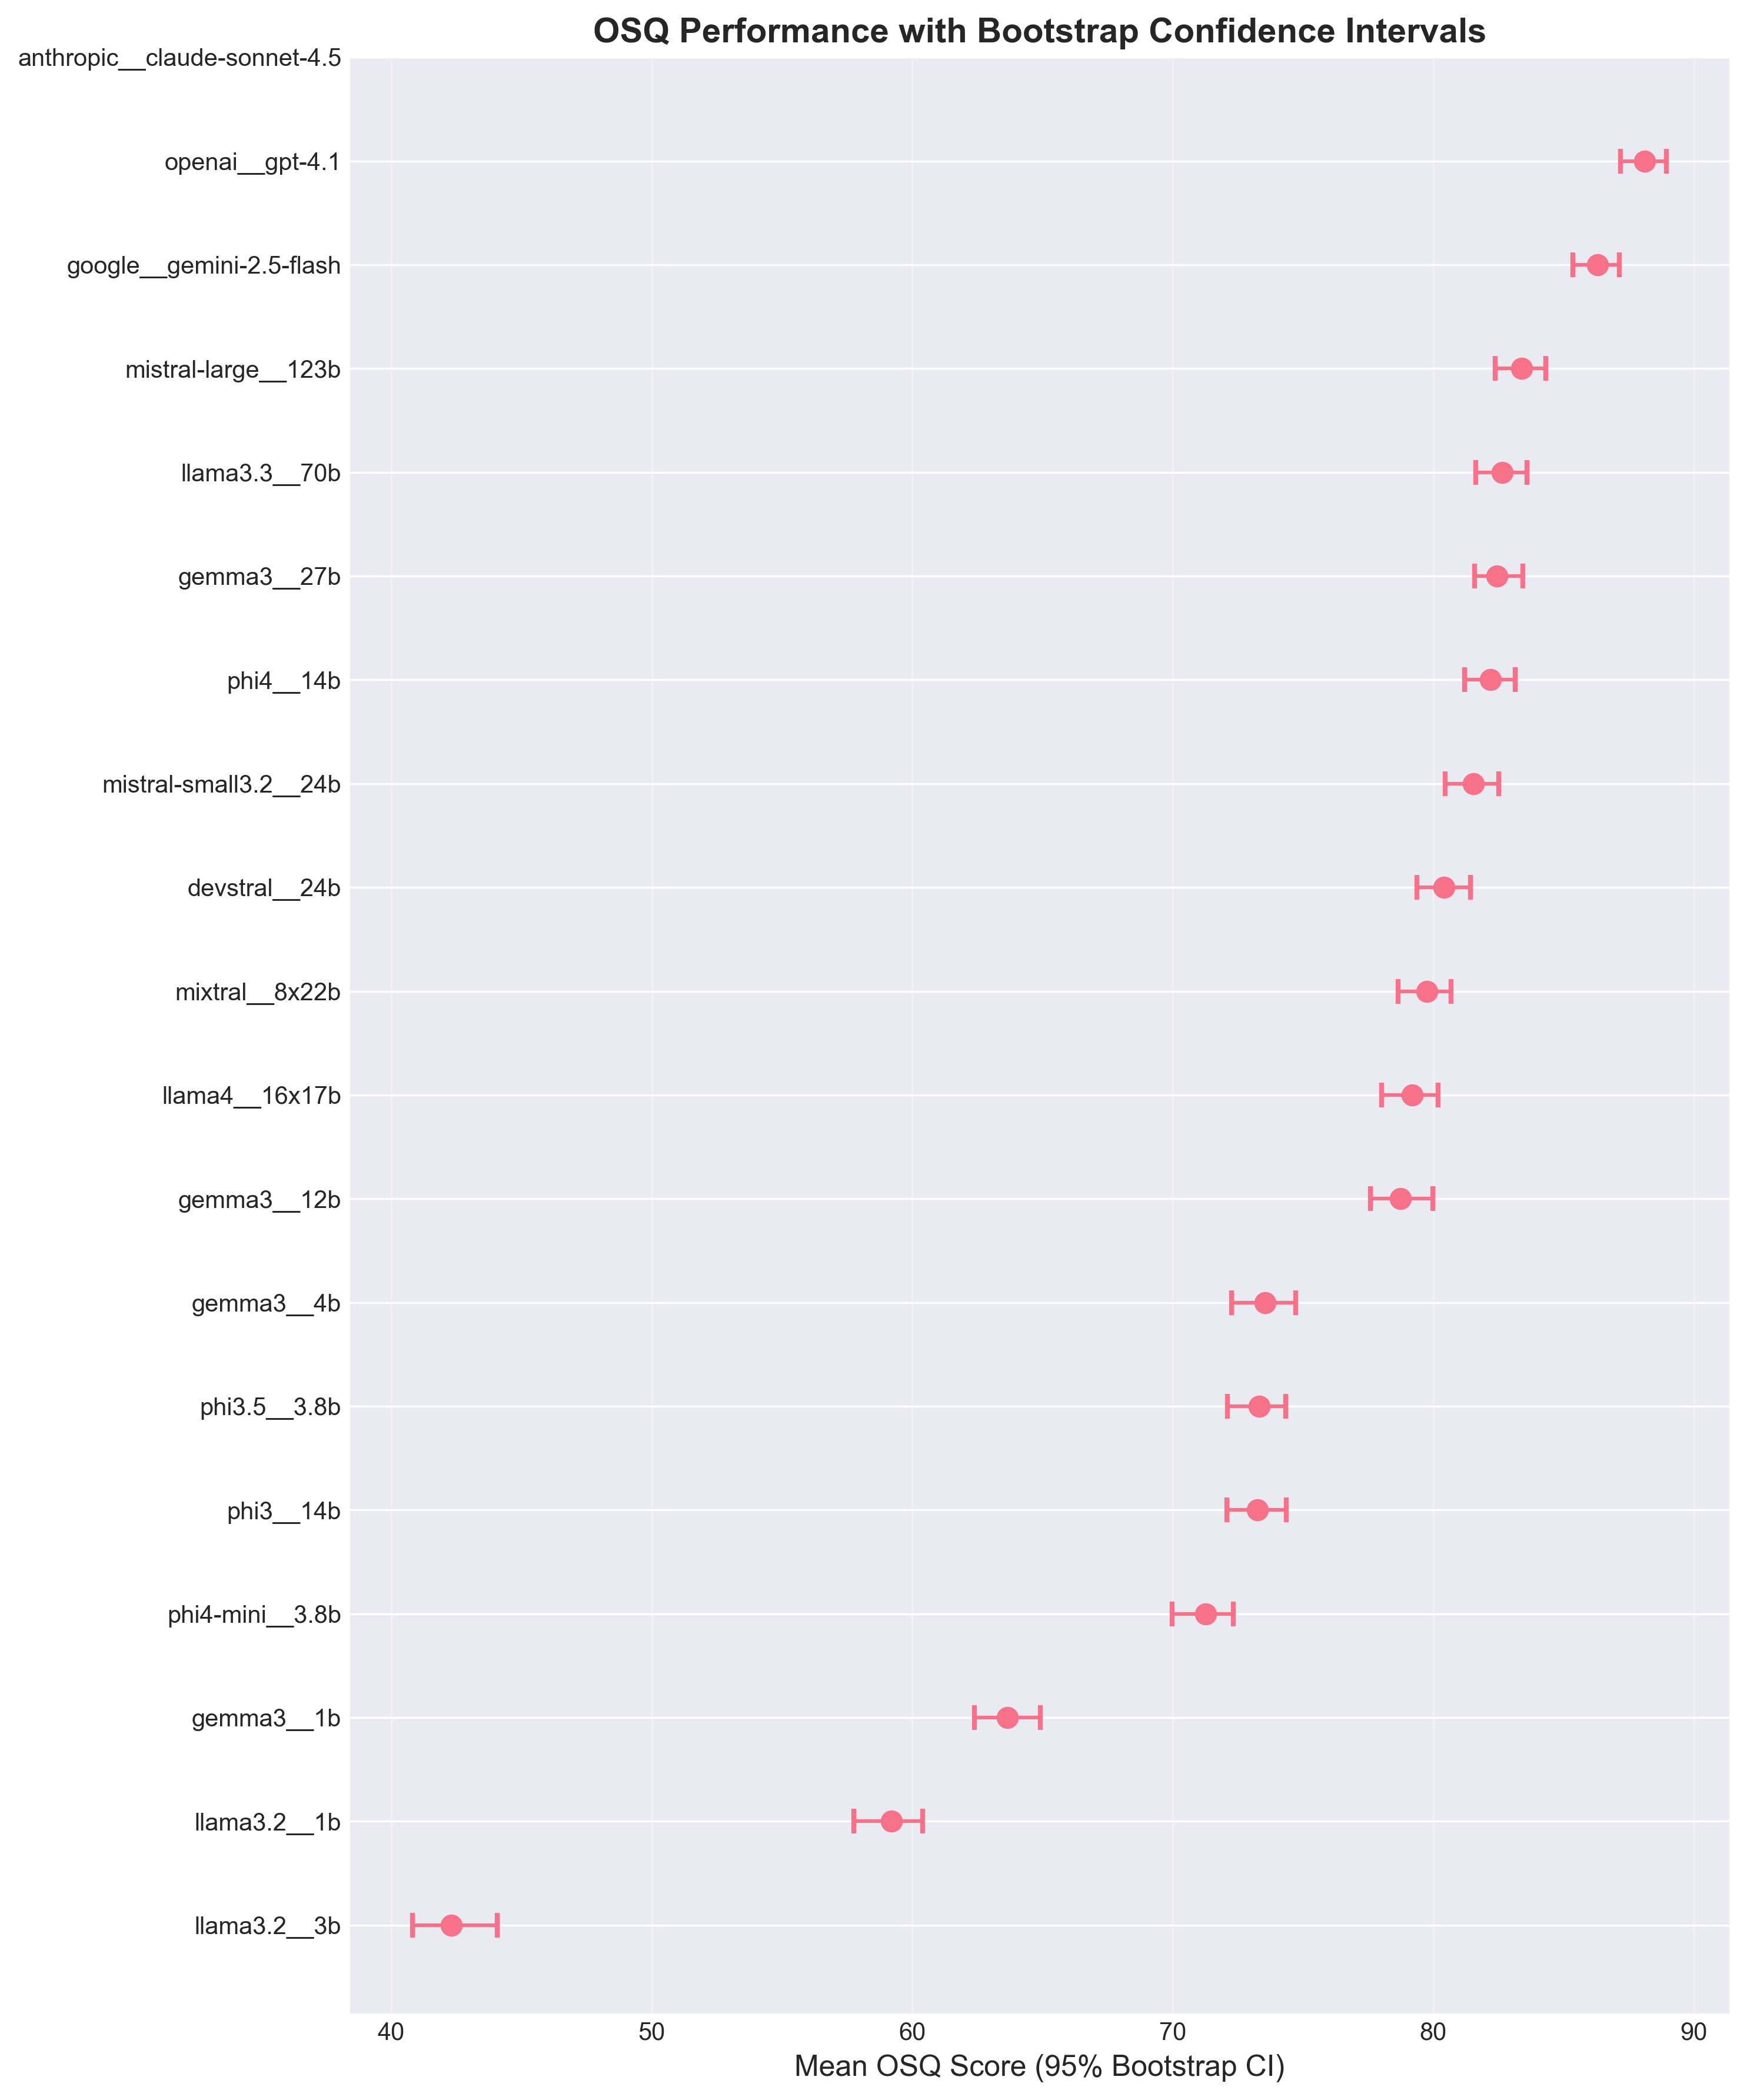
\includegraphics[width=1\linewidth]{figs/ch4/4.3/fig_osq_bootstrap_ci.png}
    \caption{OSQ Bootstrap 95\% Confidence Intervals by Model}
    \label{fig:osq_bootstrap_ci}
\end{figure}

The confidence interval widths range from approximately 1.8 to 3.2 points, with higher-performing models generally showing narrower intervals. This reflects both the score distribution characteristics and the sample sizes for each model. The intervals provide a quantitative measure of the precision of the mean OSQ score estimates.

\subsection{Performance by Bloom's Taxonomy Level}

Table \ref{tab:blooms_performance} presents OSQ performance stratified by Bloom's taxonomy cognitive level. Questions were classified during the MCQ-to-OSQ conversion process as requiring \emph{Remember}, \emph{Understand}, or \emph{Apply} level cognitive processing.

\begin{table}[htbp]
\centering
\caption{OSQ Performance by Bloom's Taxonomy Level}
\label{tab:blooms_performance}
\begin{tabular}{lrrrrr}
\toprule
Bloom's Level & Mean & Std Dev & Count & CI Lower & CI Upper \\
\midrule
Apply & 88.71 & 22.07 & 38 & 80.99 & 95.19 \\
Remember & 78.50 & 26.20 & 14,134 & 78.09 & 78.91 \\
Understand & 88.96 & 18.49 & 1,841 & 88.13 & 89.78 \\
\bottomrule
\end{tabular}
\end{table}

The results indicate that models perform best on \emph{Understand} and \emph{Apply} level questions (mean scores of 88.96 and 88.71, respectively), while showing lower performance on \emph{Remember} level questions (mean score of 78.50). This counterintuitive finding may reflect that factual recall questions (Remember level) have more objectively correct answers that are easier to grade strictly, while higher-order questions allow for more partial credit based on reasoning quality.

% \newpage
\clearpage
\section{Comparison Across MCQ and OSQ Evaluation Modalities}\label{sec:comparison_evalaution_modalities}

Figure \ref{fig:mcq-vs-osq-mean-score} presents a scatter plot comparing each model's MCQ accuracy (horizontal axis) with its mean normalized OSQ score (vertical axis). Each point represents a single model, and labels are positioned adjacent to the corresponding markers. The red dotted line indicates the line of perfect agreement between MCQ and OSQ performance, representing locations where a model would achieve identical values under both modalities. A fitted linear regression line is shown in gray, accompanied by the model's coefficient of determination (R² = 0.671) and associated p-value.

Across the distribution of points, MCQ accuracy values range approximately from 0.70 to 0.98, while normalized OSQ mean scores span roughly from 0.72 to 0.95. The plot shows with several clusters appearing toward the upper-right portion of the figure. A regression line provides a summary of the linear relationship between the two axes within the evaluated subset.

\begin{figure}[htbp]
    \centering
    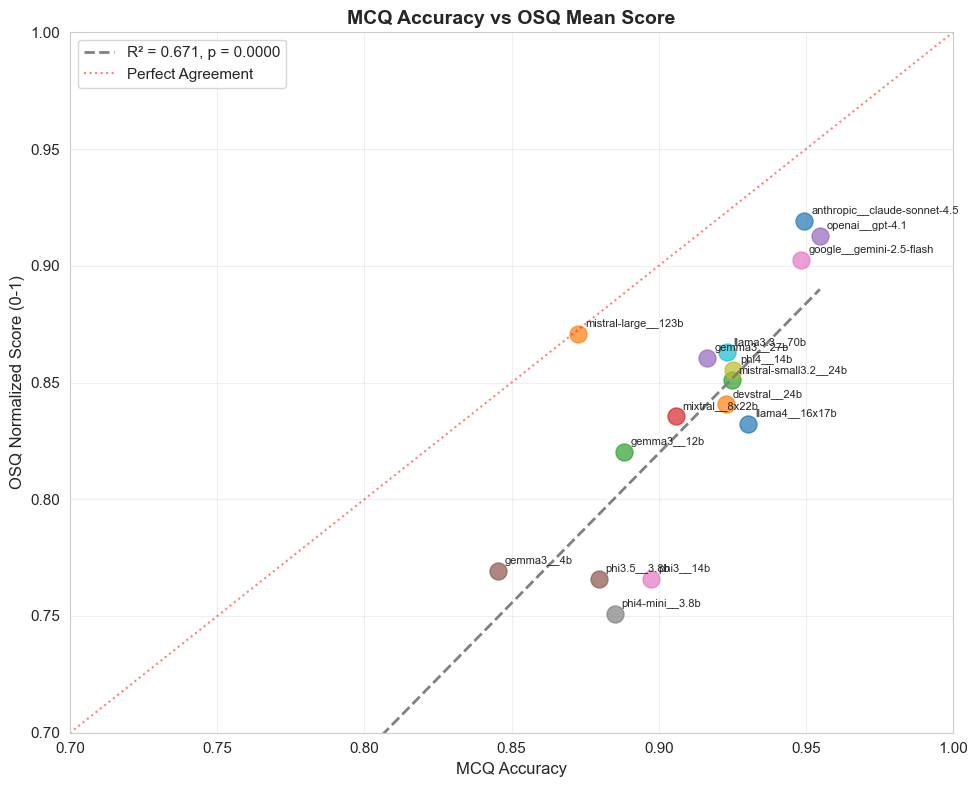
\includegraphics[width=1.00\linewidth]{figs/ch4/4.4/mcq-vs-osq-mean-score.png}
    \caption{MCQ Accuracy vs OSQ Mean Score}
    \label{fig:mcq-vs-osq-mean-score}
\end{figure}

\subsection{Correlation Analysis}

Table \ref{tab:mcq_osq_correlation} presents the correlation between MCQ accuracy and OSQ scores, computed separately for each judge model and averaged across judges. Both Pearson (linear) and Spearman (rank-order) correlations are reported.

\begin{table}[htbp]
\centering
\caption{MCQ vs OSQ Correlation Analysis}
\label{tab:mcq_osq_correlation}
\begin{tabular}{lrrrr}
\toprule
Judge & Pearson $r$ & Pearson $p$ & Spearman $\rho$ & Spearman $p$ \\
\midrule
GPT-OSS (120B) & 0.798 & $<$0.0001 & 0.800 & $<$0.0001 \\
GPT-5-mini & 0.811 & $<$0.0001 & 0.814 & $<$0.0001 \\
\textbf{Average} & \textbf{0.804} & $<$0.0001 & \textbf{0.807} & $<$0.0001 \\
\bottomrule
\end{tabular}
\end{table}

The strong positive correlations (Pearson $r$ = 0.80, Spearman $\rho$ = 0.81) indicate that MCQ accuracy is a good predictor of OSQ performance. However, the moderate R² value (0.671) also indicates that approximately one-third of the variance in OSQ scores is not explained by MCQ performance, suggesting that the two assessment formats capture partially distinct aspects of model capability.

\subsection{Statistical Test for Format Differences}

To formally test whether MCQ and OSQ scores differ systematically, Wilcoxon signed-rank tests were conducted. This non-parametric paired test compares the median difference between MCQ accuracy and normalized OSQ scores for each model. Table \ref{tab:wilcoxon_results} presents the results.

\begin{table}[htbp]
\centering
\caption{Wilcoxon Signed-Rank Test: MCQ vs OSQ}
\label{tab:wilcoxon_results}
\begin{tabular}{lrrrrr}
\toprule
Judge & Statistic & $p$-value & Median Diff & Mean Diff & $n$ \\
\midrule
GPT-OSS (120B) & 0.0 & $<$0.0001 & 0.144 & 0.160 & 19 \\
GPT-5-mini & 0.0 & $<$0.0001 & 0.076 & 0.092 & 19 \\
\textbf{Average} & 0.0 & $<$0.0001 & \textbf{0.113} & \textbf{0.126} & 19 \\
\bottomrule
\end{tabular}
\end{table}

The Wilcoxon test yields $p < 0.0001$ for both judges, indicating a statistically significant difference between MCQ and OSQ performance. The positive median difference (0.11–0.14) indicates that models systematically score higher on MCQ than on OSQ (after normalization to a 0–1 scale), suggesting that the OSQ format is more challenging or discriminating than the MCQ format.

\subsection{Effect Size Analysis}

Cohen's $d$ was computed to quantify the practical significance of the difference between MCQ and OSQ performance. Table \ref{tab:effect_sizes} presents the effect sizes for each judge and the average.

\begin{table}[htbp]
\centering
\caption{Effect Sizes for Format Comparison (Cohen's $d$)}
\label{tab:effect_sizes}
\begin{tabular}{lrrr}
\toprule
Judge & Cohen's $d$ & Interpretation & $n$ \\
\midrule
GPT-OSS (120B) & 2.35 & Large & 19 \\
GPT-5-mini & 1.30 & Large & 19 \\
\textbf{Average} & \textbf{1.82} & \textbf{Large} & 19 \\
\bottomrule
\end{tabular}
\end{table}

The large effect sizes (Cohen's $d$ = 1.30–2.35) indicate that the difference between MCQ and OSQ performance is not only statistically significant but also practically meaningful. By conventional interpretation, a Cohen's $d$ greater than 0.8 represents a large effect. The observed effect sizes substantially exceed this threshold, confirming that the assessment format (MCQ vs OSQ) has a substantial impact on measured model performance.

\subsection{MCQ vs OSQ Rubric Dimension Correlation}

Figure \ref{fig:mcq_osq_rubric_dimensions} presents the relationship between MCQ accuracy and each of the five OSQ rubric dimensions. This analysis reveals which aspects of OSQ performance are most strongly predicted by MCQ accuracy.

\begin{figure}[htbp]
    \centering
    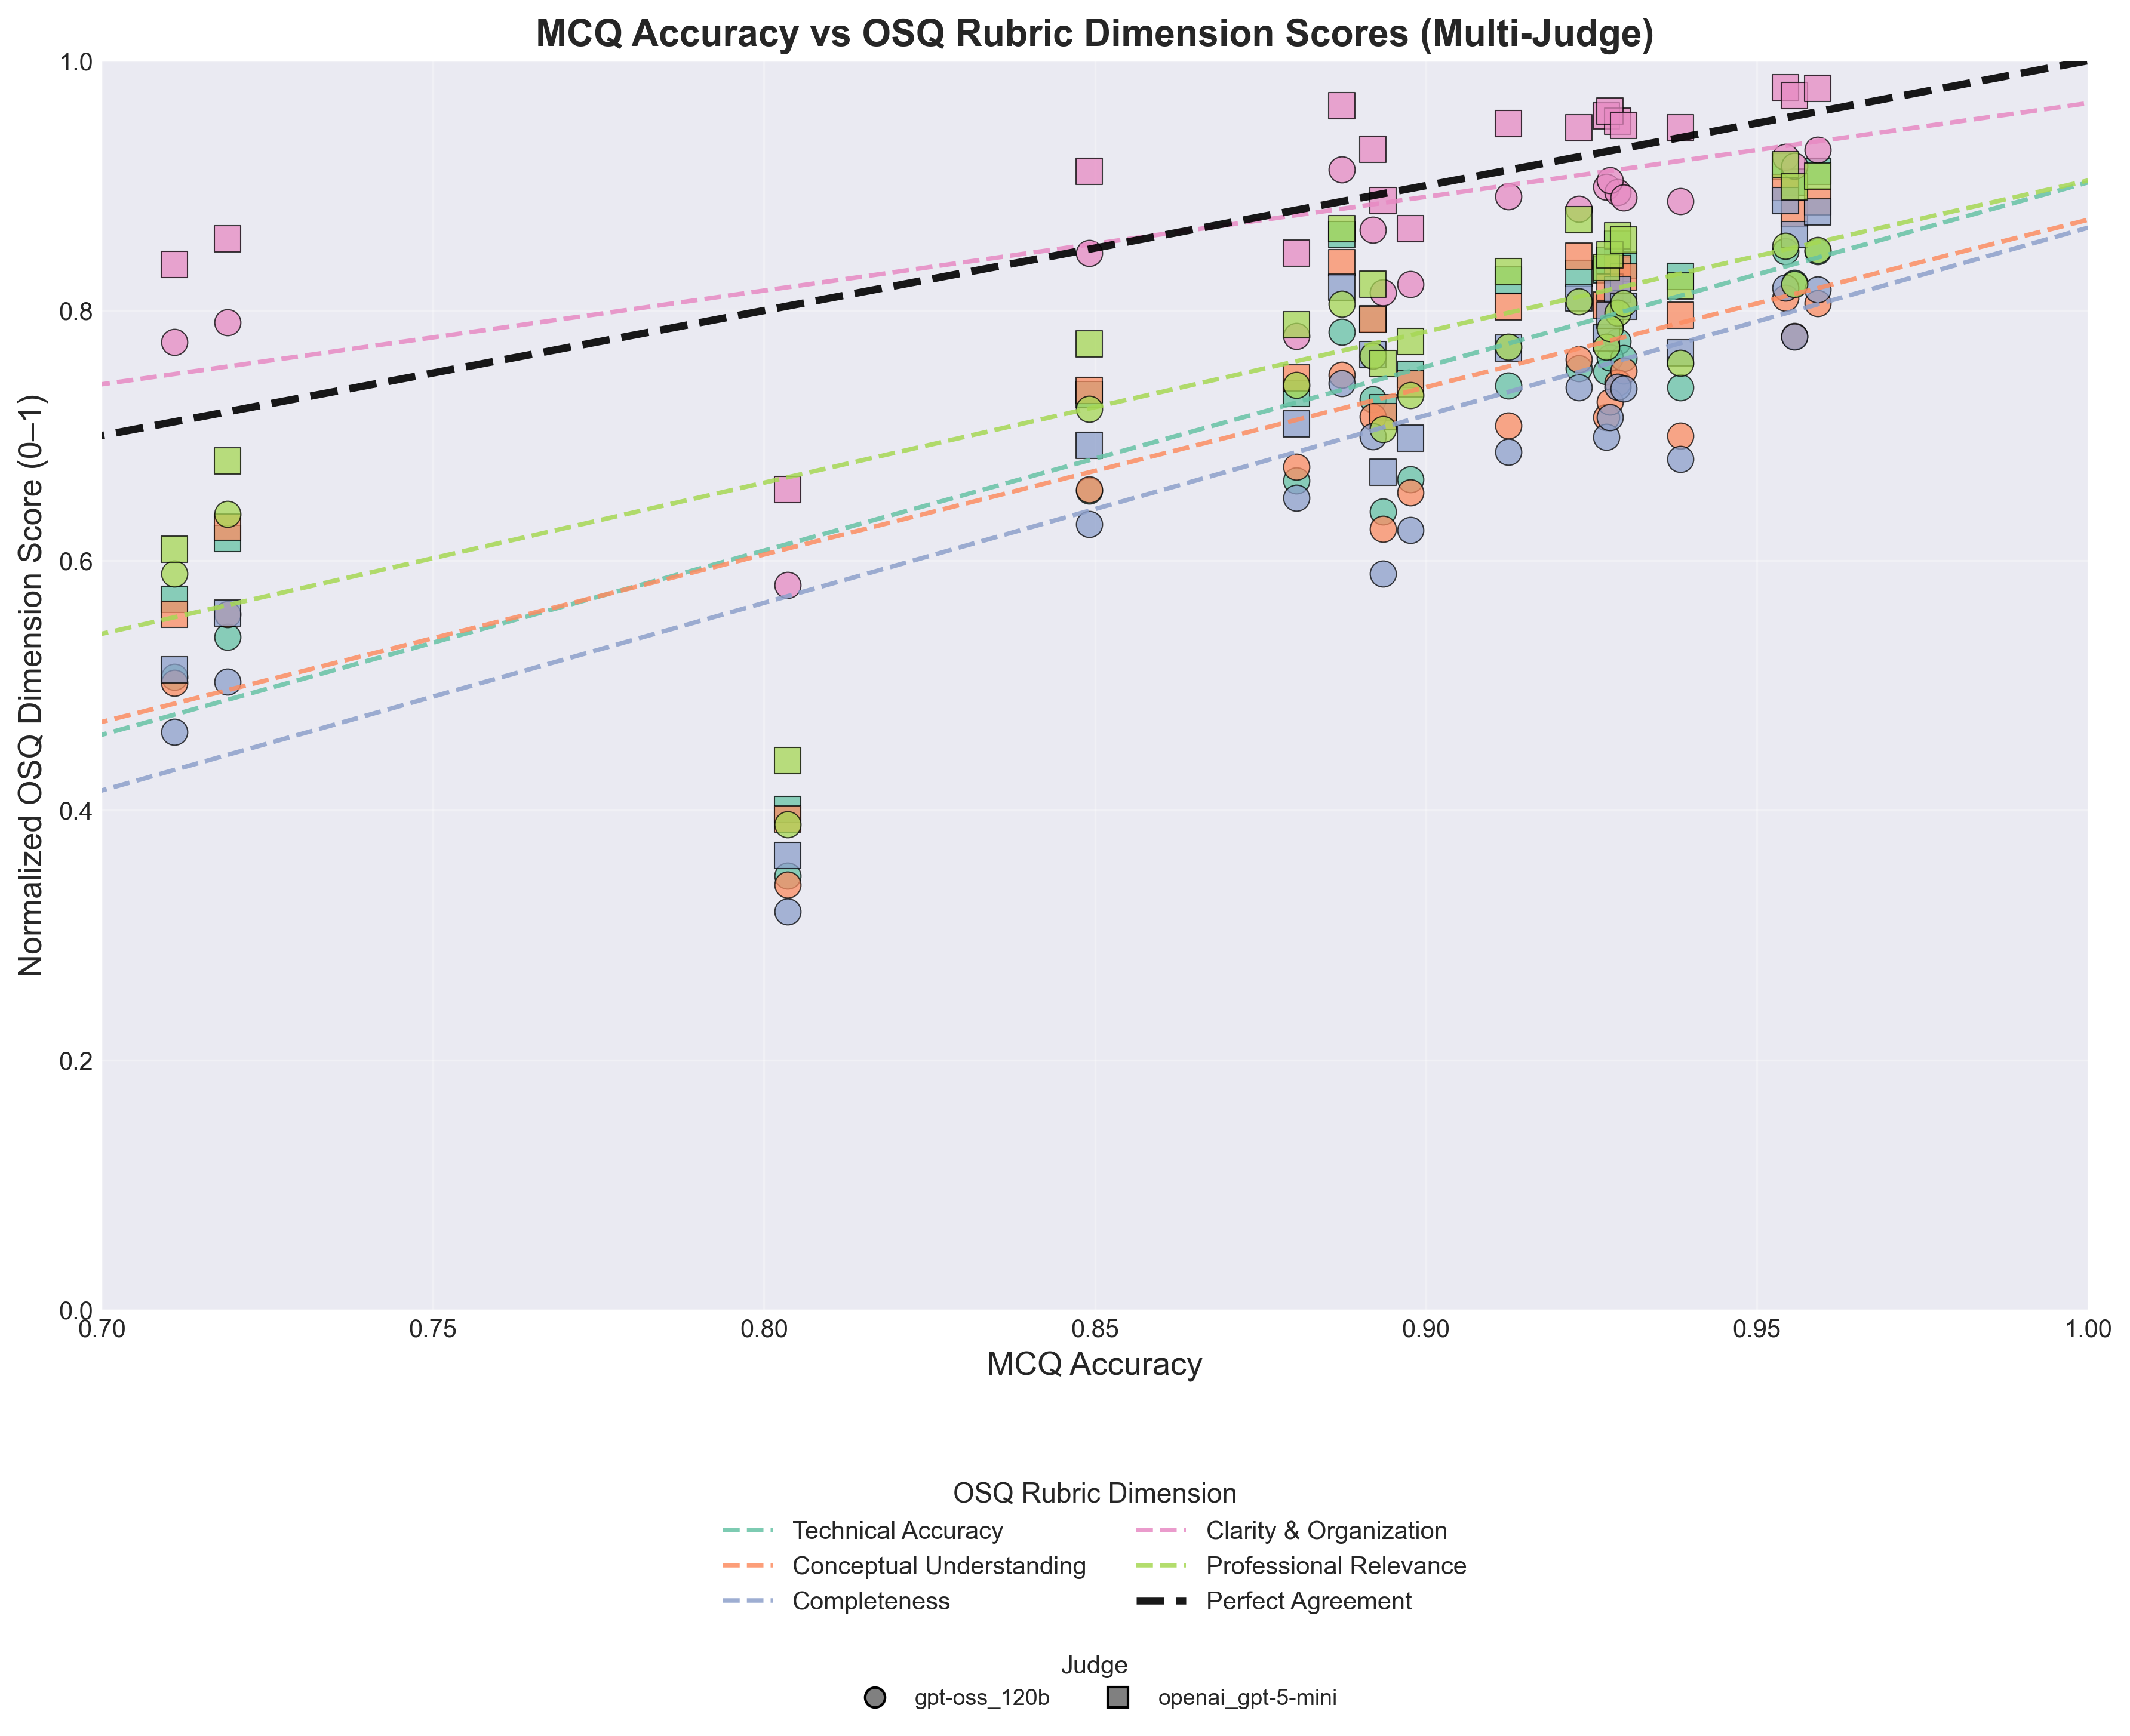
\includegraphics[width=1\linewidth]{figs/ch4/4.4/mcq_vs_osq_rubric_combined_multijudge.png}
    \caption{MCQ Accuracy vs OSQ Rubric Dimensions (Multi-Judge)}
    \label{fig:mcq_osq_rubric_dimensions}
\end{figure}

% \newpage
\clearpage
\section{Tokenomics and Cost}\label{sec:tok}

The top panel of Figure \ref{fig:tokenomics_distribution} shows violin plots illustrating the distribution of response token counts for each evaluated model. Models are displayed along the horizontal axis, and response length in tokens is plotted on the vertical axis. Each violin represents a kernel density estimate of token usage for that model, with wider regions indicating more frequently occurring token counts. The embedded box plot within each violin highlights the median, inter-quartile range, and approximate overall spread.

Across models, response token counts range from fewer than 20 tokens to more than 500 tokens. Several models display relatively compact distributions centered near shorter responses, while others show broader or more elongated violins indicative of greater variability in response length. A number of models include long upper tails reflecting occasional high-token responses. The prompt was limited to 500 tokens maximum, with recommendations for 1-2 sentence responses by default, with few question prompts for 3-4 sentence responses.

\begin{figure}[htbp]
    \centering
    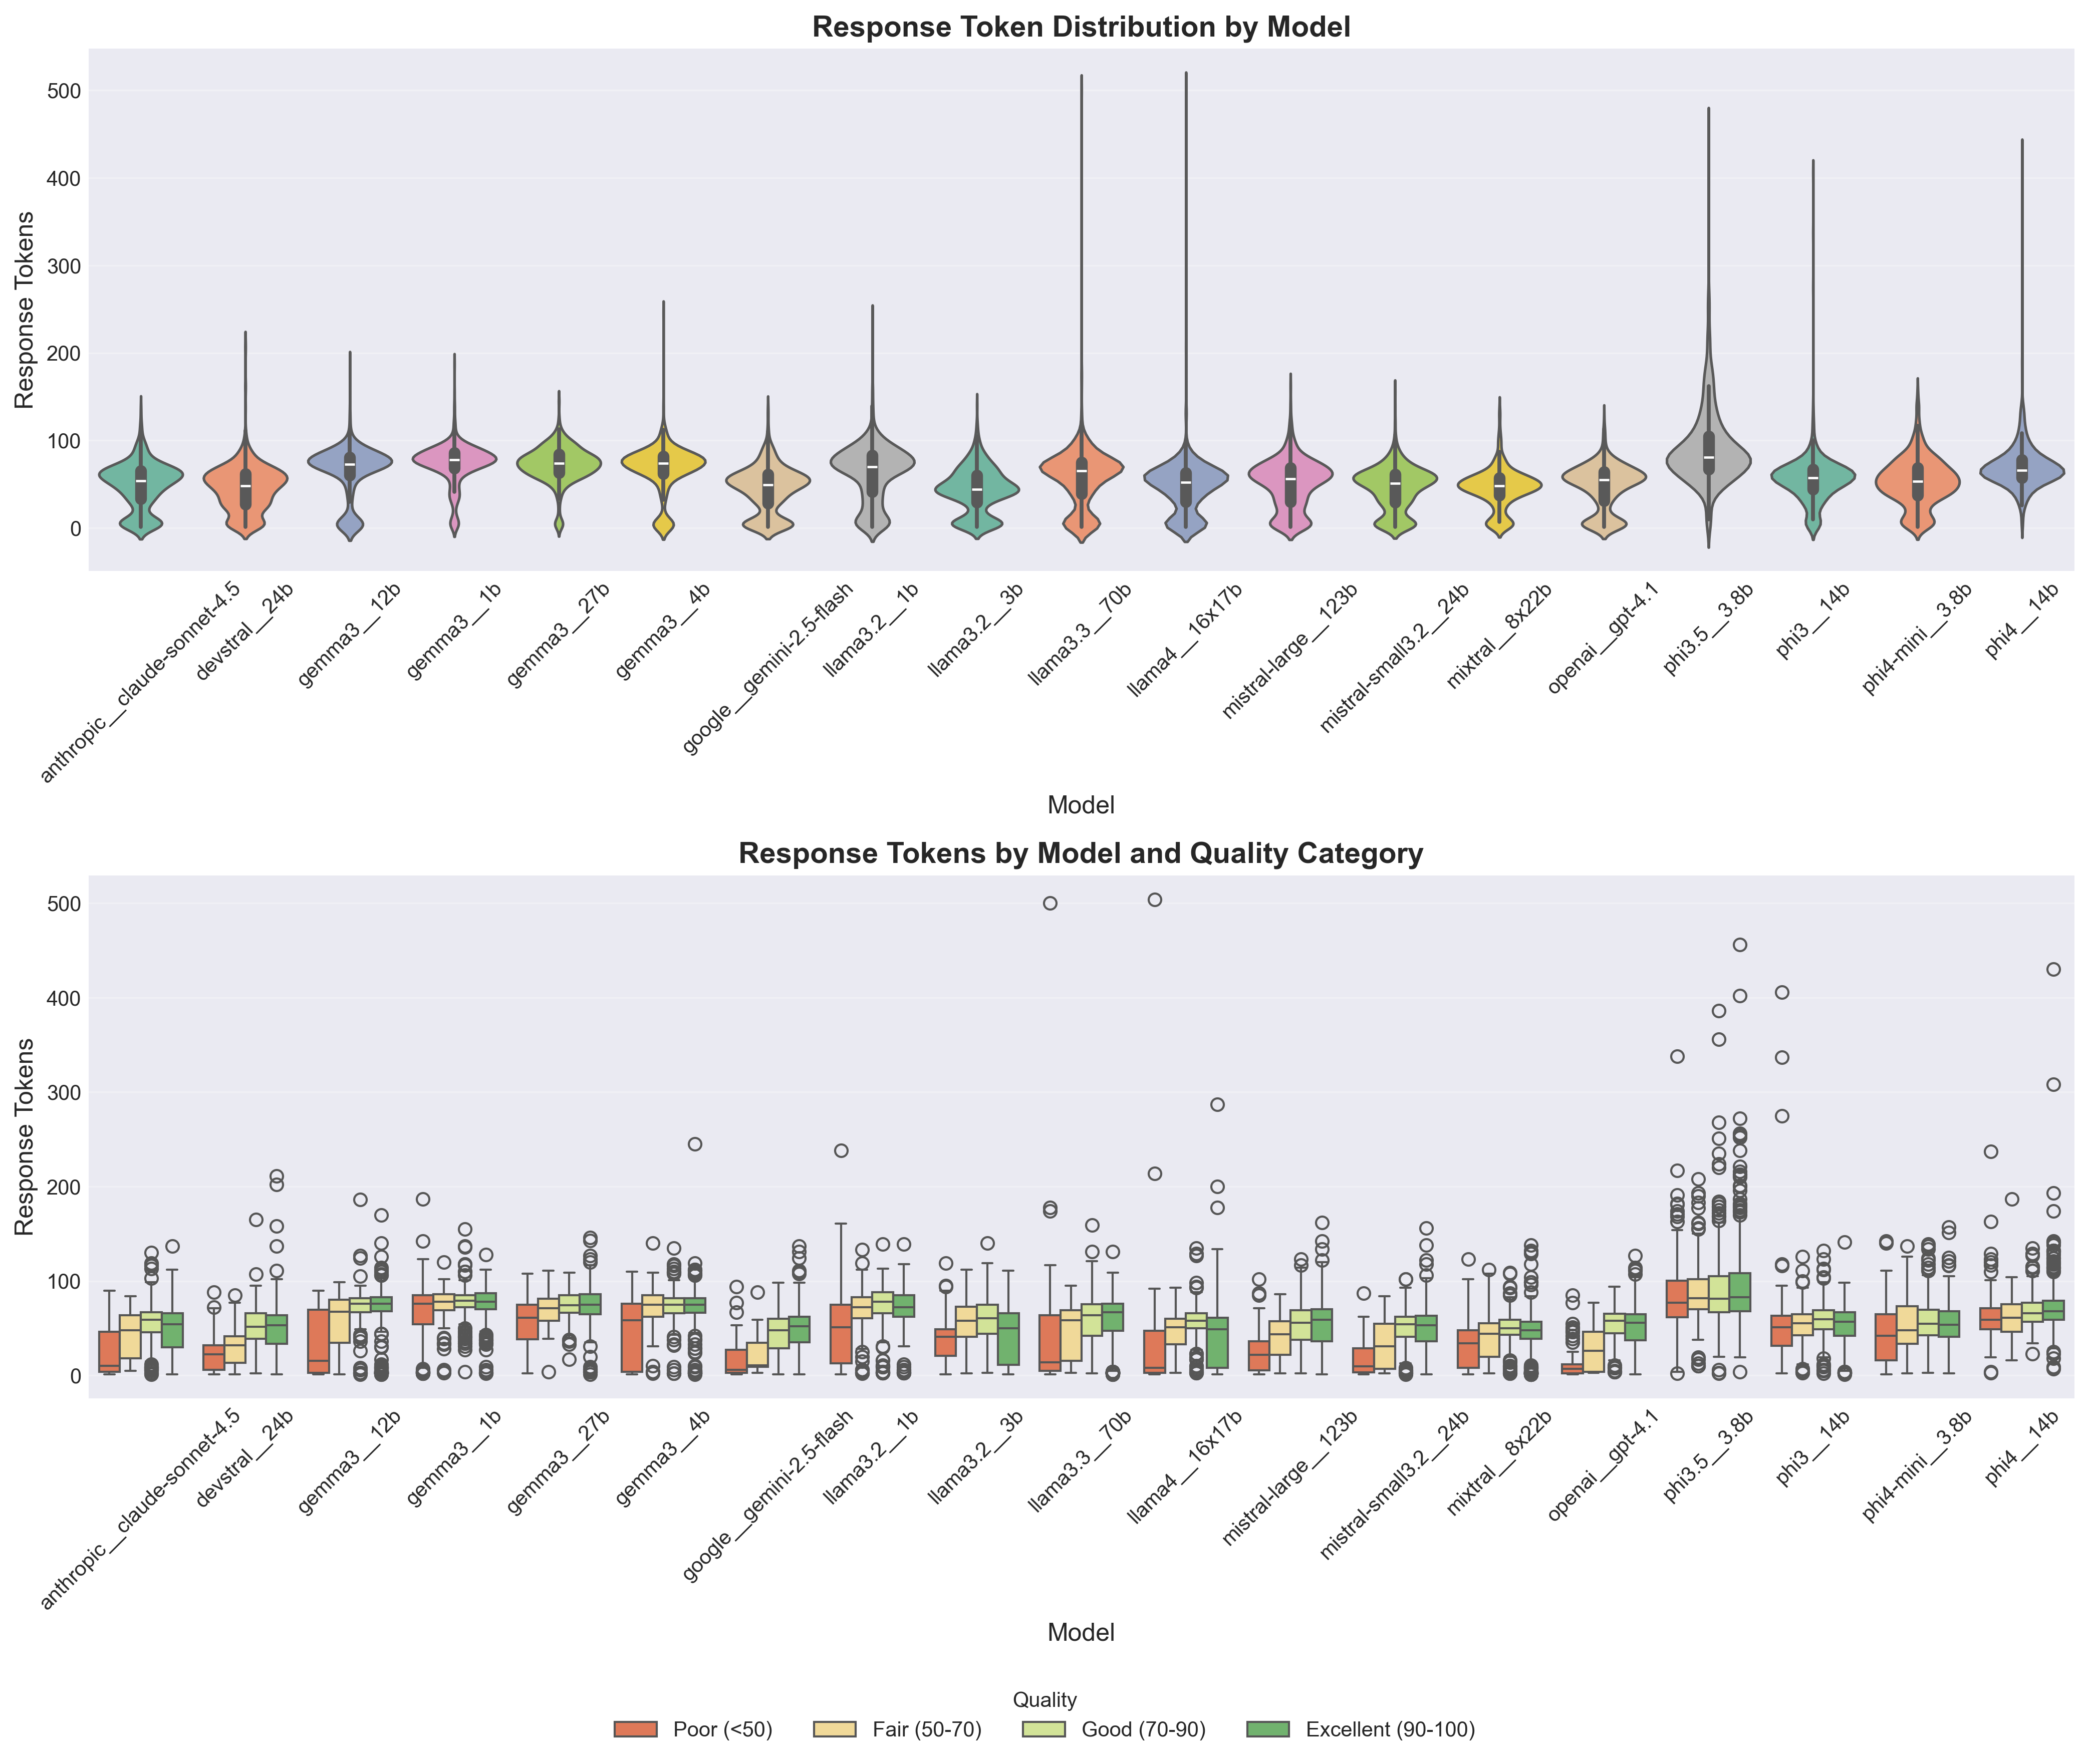
\includegraphics[width=1\linewidth]{figs/ch4/4.5/tokenomics_distribution.png}
    \caption{Response Token Distribution by Model}
    \label{fig:tokenomics_distribution}
\end{figure}

\subsection{Quality-Efficiency Trade-offs}

Figure \ref{fig:response_tokens_quality} presents response token counts stratified by quality tier, revealing the relationship between verbosity and response quality across models.

\begin{figure}[htbp]
    \centering
    
\includegraphics[width=1\linewidth]{figs/ch4/4.5/response_tokens_by_model_and_quality_avg_judge.png}
    \caption{Response Tokens by Model and Quality Tier}
    \label{fig:response_tokens_quality}
\end{figure}

\subsection{Pareto Efficiency Analysis}

Figure \ref{fig:pareto_frontier} presents a Pareto efficiency analysis of model performance, plotting mean OSQ score (quality) against mean response token count (cost proxy). Models on the Pareto frontier achieve the best quality-to-cost trade-off---no other model offers higher quality at the same or lower token usage.

\begin{figure}[htbp]
    \centering
    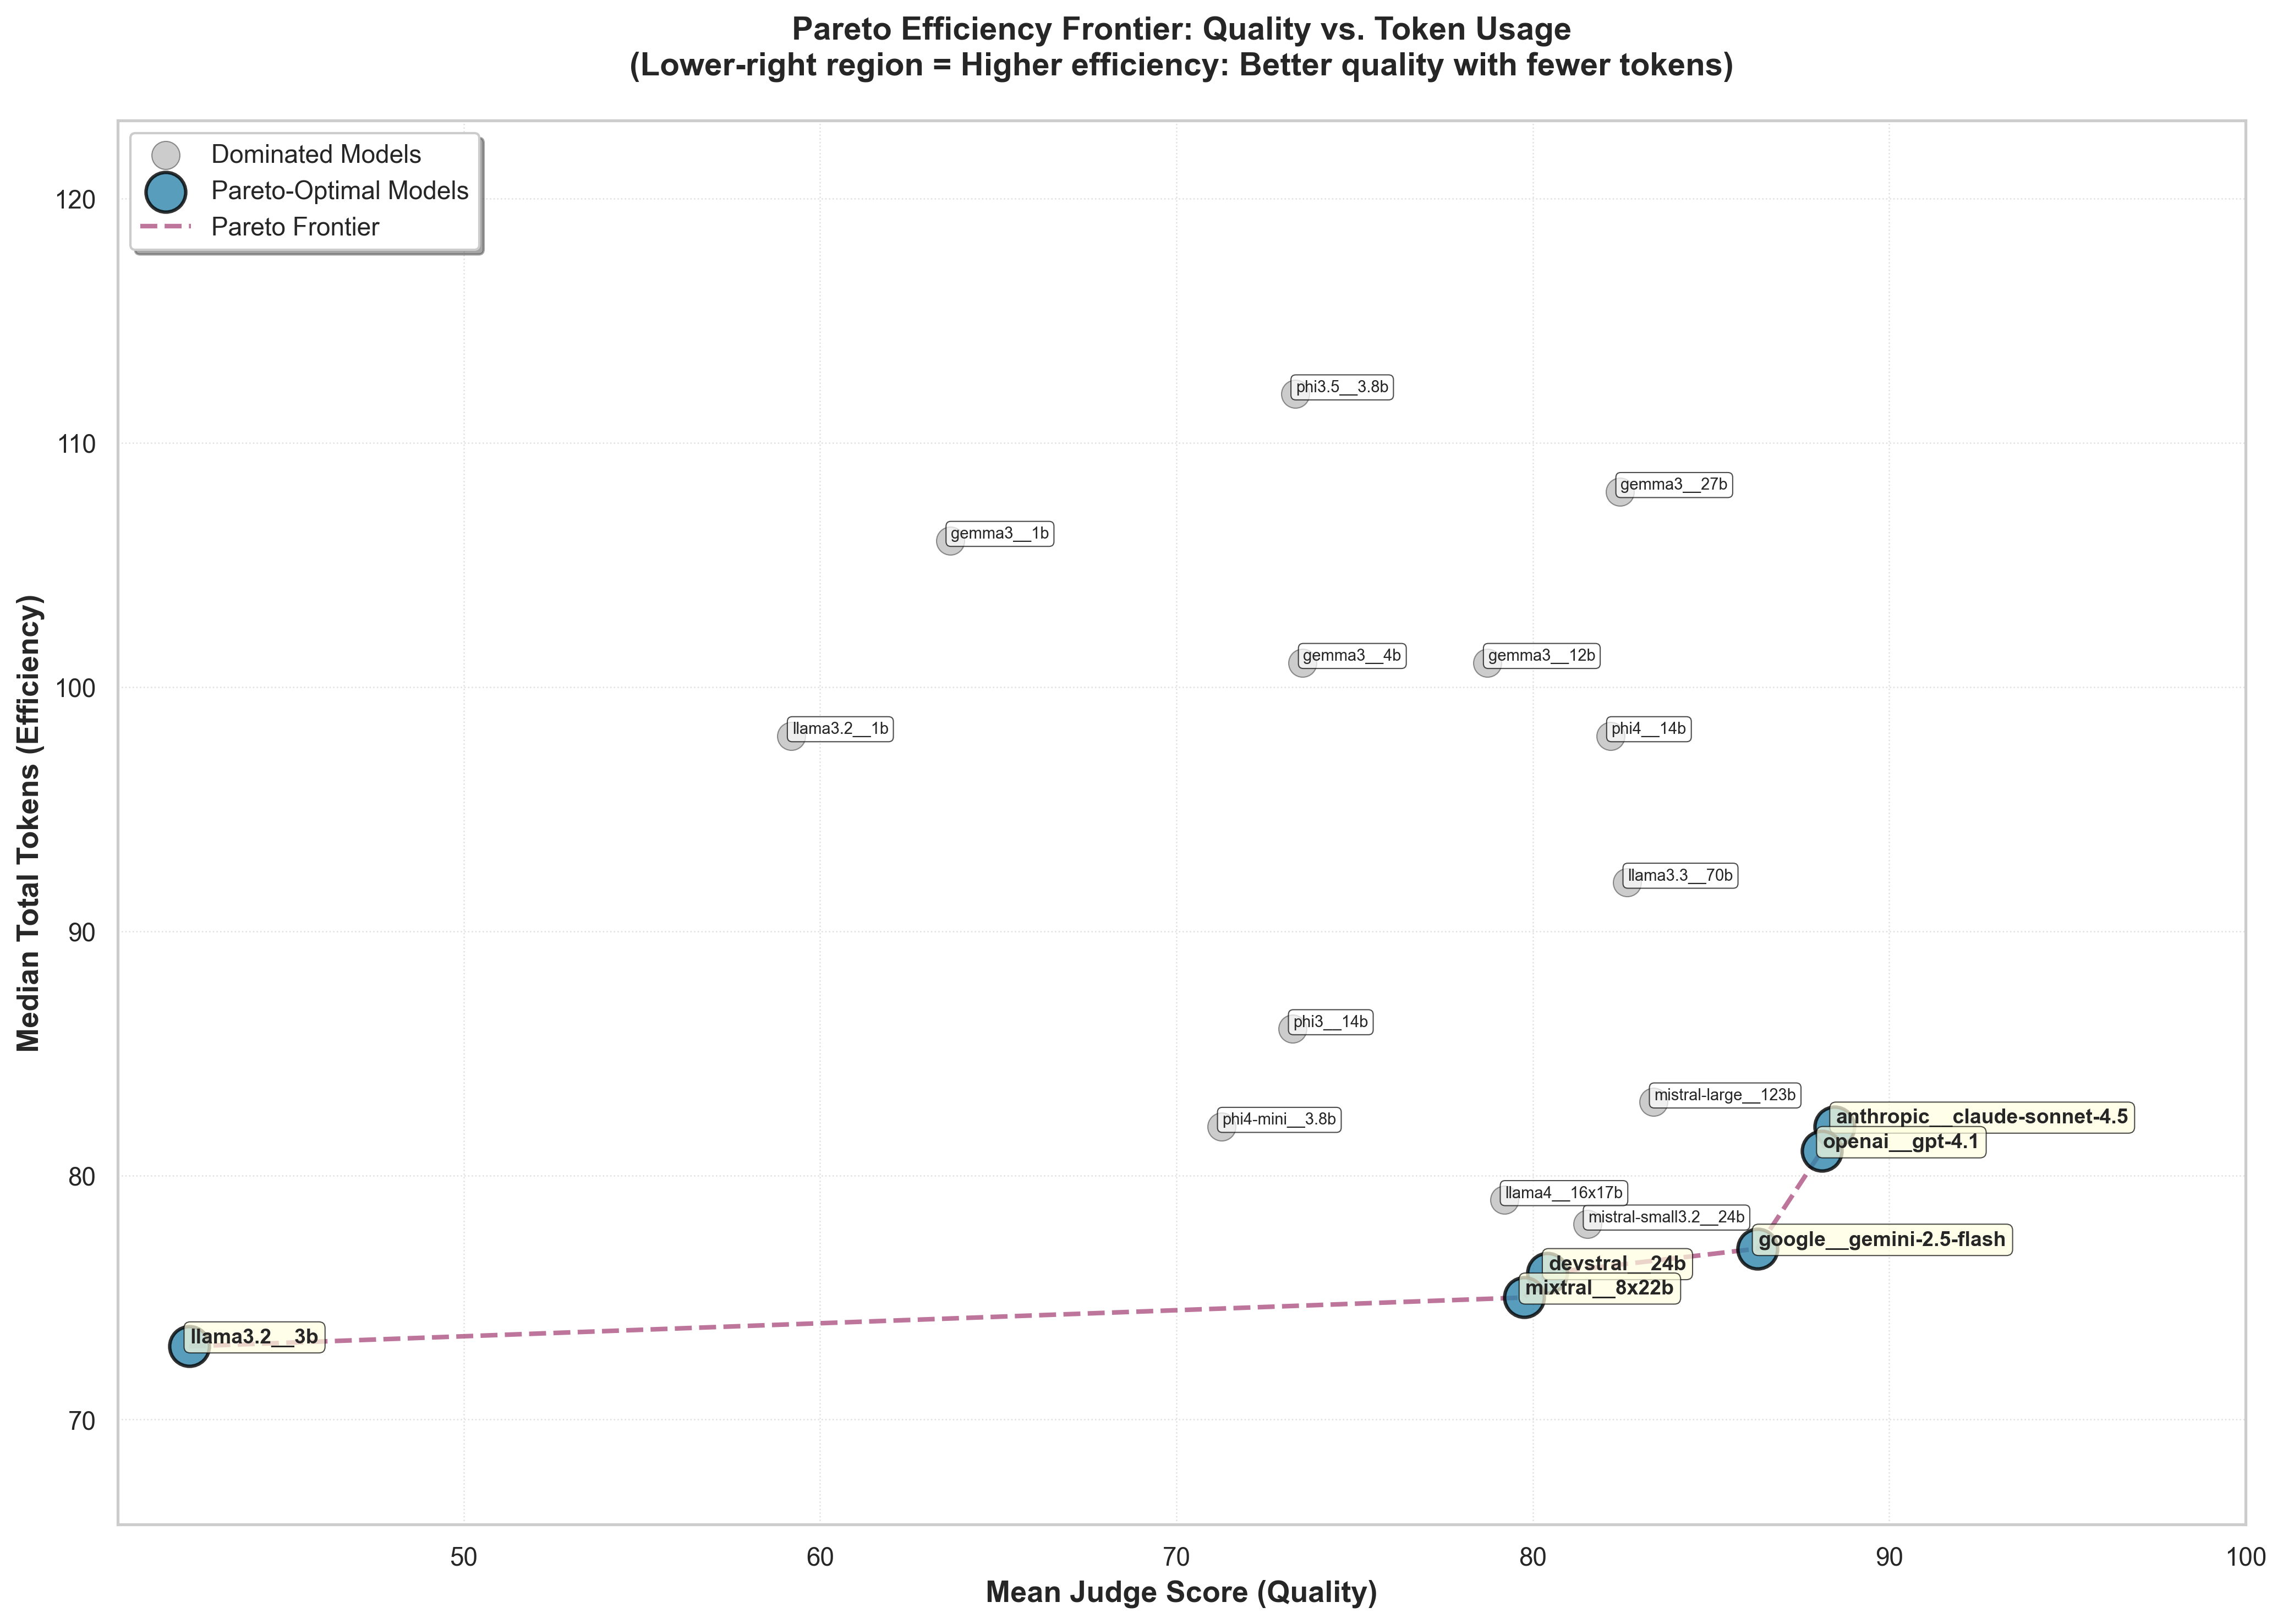
\includegraphics[width=1\linewidth]{figs/ch4/4.5/pareto_efficiency_frontier.png}
    \caption{Pareto Efficiency Frontier: Quality vs Token Usage}
    \label{fig:pareto_frontier}
\end{figure}

The Pareto frontier identifies models that represent optimal trade-offs between quality and efficiency. Models below the frontier are dominated by at least one other model that achieves equal or higher quality with equal or fewer tokens. This analysis provides practical guidance for model selection based on resource constraints and quality requirements.
